\chapter{Etablierung Agiler Praktiken}
\label{agilepractices}

% - erkenntnisreichster Teil der Arbeit!
% - Erarbeitung von verwendeten agilen Praktiken
% - Evaluation hinsichtlich ihrer Anwendbarkeit bei den vorher erarbeiteten Problemfeldern

Im nachfolgenden Kapitel soll der zweite wesentliche Schwerpunkt der vorliegenden Arbeit erarbeitet werden. Nachdem in \ref{problemfields} grundsätzliche Problemfelder innerhalb der Digitalen Transformation von Großunternehmen untersucht wurden, sollen nun anhand eines zweiten SLR agile Methoden gefunden werden, die diesen Problemfeldern begegnen können. Als erster Schritt soll wiederum das methodische Vorgehen erläutert werden, wonach eine Reihe von Literatur für das zweite SLR zusammengestellt wurde. Anhand dieser werden agile Methoden extrahiert, die vermehrt innerhalb des Transformationsprozesses eingesetzt wurden. Diese sollen anschließend kurz dargestellt und hinsichtlich ihrer Anwendbarkeit bei bestimmten Problemfeldern evaluiert werden. Als Ergebnis dessen sollen als generelles Resultat der vorliegenden Arbeit Best Practices für den Einsatz agiler Methoden in der Digitalen Transformation ausgearbeitet werden. Das nachfolgende Literaturreview wird durch das Akronym \textit{SLR 2} abgekürzt.

\section{Methodisches Vorgehen}
\label{agilepractices:methods}

% - genaue Darstellung über Vorgehen in der SLR + Metastudie: 
% - Suchmethodik, Keywords, Kriterien, Auswahlprozes ...
% + Schema der Evaluation (Problemfelder)
% https://docs.google.com/document/d/1j8hegu3FgQk2fPMVjo8IUPWIXwNjlZjT42rHxg7KZ1I/edit

Das Vorgehen in den folgenden Ausführungen teilt sich in zwei wesentlichen Unterpunkten. Zunächst soll, ähnlich dem SLR 1 in \ref{problemfields}, ein systematisches Literaturreview mit Metastudiencharakter vorgenommen werden. Die Vorgehensweise ähnelt der des ersten SLR, etwaige Besonderheiten werden nachfolgend aufgeführt. Der zweite  methodische Teil beinhaltet die Evaluation der erarbeiteten agilen Methoden. Dafür soll ebenfalls nachfolgend ein Evaluationsschema skizziert werden.

\subsection{Systematisches Literaturreview}

Im Vorfeld der Literatursuche wurde zunächst eine Suchstrategie erstellt. Diese ähnelt der im \ref{problemfields:methods} dargestellten, \ref{fig:suchstrategie} illustriert somit ebenfalls die Strategie zur Suche relevanter Literatur für SLR 2. Für die zweite Literatursuche wurden die verwendeten Keywords verändert. Wiederrum wurden diese in Suchketten zusammengefasst, welche sich jeweils für englische und deutsche Literaturdatenbanken unterscheiden. Die genutzten Suchketten werden in \ref{tab:keywordsslr2} aufgeführt. An dieser Stelle sei wieder zu erwähnen, dass die Syntax zwischen verschiedenen Suchmaschinen unterscheiden kann. Die Übersicht dient der Allgemeinheit.

\begin{table}[ht]
	\centering
	\caption{Übersicht Keyword-Suchketten SLR 2}
	\begin{tabular}{|p{7cm}|p{7cm}|}
		\hline
		\textbf{Deutsche Keywords}& \textbf{Englische Keywords} \\
		\hline
		agile+transformation+fallstudie OR digitale+transformation+agil OR agile+organisation+fallstudie   & agile+transformation+case OR digital+transformation+agile OR agile+organization+case \\
		\hline
	\end{tabular}
	\label{tab:keywordsslr2}
\end{table}

Auch die verwendeten Literaturdatenbanken bzw. Suchmaschinen ähneln denen des ersten SLR. Wiederrum wurde eine Übersicht für die Anzahl an Treffern der Keywords in den jeweiligen Suchmaschinen aufgestellt. Diese findet sich in \ref{tab:suchmaschinenslr2}. Für die Suchmaschine \textit{ResearchGate} konnte auch für die zweite Literatursuche keine Angabe zu Keyword-Treffern gemacht werden. Eine kurze Erklärung findet sich in \ref{problemfields:methods}.

\begin{table}[ht]
	\centering
	\caption{Übersicht Literatursuchmaschinen SLR 2}
	\begin{tabular}{|p{5cm}|p{7cm}||p{3cm}|}
		\hline
		\textbf{Datenbank/Bibliothek}& \textbf{URL} &  \textbf{Treffer Keywords  (summiert)} \\
		\hline
		IEEE Xplore & \url{https://ieeexplore.ieee.org} & 316 \\
		(Online) - Bibliothek Hochschule Harz & \url{https://opac.lbs-magdeburg.gbv.de/DB=4/LNG=DU} & 4 \\
		(Online) - Bibliothek Technische Universität Berlin  & \url{https://www.ub.tu-berlin.de/literatur-suchen}& 5 \\
		Google Scholar &  \url{https://scholar.google.de}  & 23.500 \\
		Scopus & \url{https://www.scopus.com} & 1.491 \\
		ResearchGate & \url{https://www.researchgate.net} &Keine Angabe vorhanden \\ 
		ACM Digital Library & \url{https://dl.acm.org} & 251.254 \\
		\hline
	\end{tabular}
	\label{tab:suchmaschinenslr2}
\end{table}

Die andauernde Literatursuche wurde wieder mithilfe einer Forwards-Backwards-Suche unterstützt. Die angestrengte Suche erzielte somit wieder eine große Menge an potenzieller Literatur zur Thematik. Somit war auch hier eine Filterung der Ergebnisse mithilfe eines Auswahlprozesses notwendig. Dieser gleicht ebenfalls der im ersten SLR. Somit zeigt \ref{fig:auswahlprozess} in \ref{problemfields:methods} eben diesen. 

Auch für dieses Auswahlprozedere wurden eine Reihe von Ein - und Ausschlusskriterien definiert. Diese werden nachfolgend in \ref{tab:criteriaslr2}. Auch hier zeigen sich verständlicherweise Parallelen zum ersten SLR. Wichtig hier zu erwähnen sei, dass innerhalb der Publikationen ein klarer Bezug zu agilen Methoden im Transformationsprozess erkennbar sein muss. Hierbei reicht nicht nur die Nennung einzelner Methoden, es muss klar ersichtlich sein, welchen Beitrag diese zum Veränderungsprozess beigetragen werden. Dies ist gerade wichtig im Hinblick auf die nachfolgende Evaluation. Im Bezug auf Internationalität und Branchenzugehörigkeit wurden keine Einschränkungen getroffen.

\begin{table}[ht]
	\centering
	\caption{Ein - und Ausschlusskriterien SLR 2}
	\begin{tabular}{|p{4cm}|p{8cm}|}
		\hline
		\textbf{Kriterium}& \textbf{Erklärung}  \\
		\hline
		Empirik & Literatur muss eine Fallstudie oder Studie sein. Fachliteratur auch dann möglich, wenn klarer Bezug auf Agile Organisationsentwicklung in Großunternehmen \\
		Wissenschaftlichkeit & Methodik der  Fallstudie oder Studie muss klar erkennbar sein \\
		Kontext 1 & inhaltlich Digitale Transformation in Großunternehmen; Mittelständische nur dann, wenn relevant für größeren Kontext \\
		Kontext 2 & Nutzung klarer, spezifischer agiler Methoden im Transformationsprozess \\
		Sprache & deutsch oder englisch \\
		Aktualität & ab 2014 - heute  \\
		\hline
	\end{tabular}
	\label{tab:criteriaslr2}
\end{table}

Durch eine zweite Literatursuche konnte wieder eine große Menge relevanter Literatur, in diesem Falle nicht vollumfänglich Fallstudien, für die nachfolgenden Untersuchungen erschlossen werden. Zwischen beiden Untersuchungen gab es in der Ergebnismenge Überschneidungen, da manche Fallstudien ebenfalls die Nutzung agiler Methoden einschlossen. Dies ist deshalb sehr interessant, weil dadurch direkt Handlungsfelder agiler Methoden hinsichtlich der geschilderten Problemfelder erkennbar wurden. Insgesamt konnten nach dem Auswahlprozess \textit{32} Publikationen für die weitere Verwendung gefunden werden. Darunter beinhalten 29 davon Fallstudien, 3 sind Fachliteratur. Die Anzahl der Fallstudien konnte diesmal auf über \textit{180} aus verschiedenen Branchen gezählt werden. An den eingeschlossenen Studien nahmen insgesamt über 1500 Offizielle aus Großunternehmen teil. 

\subsection{Evaluation}
\label{agilepractices:evaluationschema}

Als zweiter methodischer Teil wurde eine Evaluation der zuvor erarbeiteten agilen Methoden vorgesehen. Diese soll nach einem klaren Schema erfolgen, welches nachfolgend erläutert werden soll. 

Die vorgenommene Evaluation wurde nach Vorbild eines Leitfadens des Bundesministerium für Ernährung und Landwirtschaft erstellt \footnote{Leitfaden Evaluation, \newline online: \url{https://www.in-form.de/fileadmin/Dokumente/Materialien/IN_FORM_Leitfaden_Evaluation.pdf}}. Dieser beinhaltet insgesamt 6 Phasen, welche in \ref{fig:evaluation} dargestellt werden. Zu jeder Phase zeigt die Abbildung ebenfalls das Resultat im Bezug auf die  vollzogene Evaluation. 

Zunächst sollte das Ziel der Evaluation dekliniert werden. Im Vordergrund stand hierbei ganz klar die Lösung der in \ref{problemfields} erarbeiteten Problemfelder. Anschließend wurde der  Evaluationsgegenstand bestimmt. Dieses findet sich in der mithilfe des SLR 2 gefundenen agilen Praktiken bzw. Methoden. Somit setzt sich das zu betrachtende Untersuchungsfeld der Evaluation aus einer Beziehung zwischen Problemfelder der Digitalen Transformation und agilen Methoden zusammen.

\begin{figure}[H]
	\centering
	\fbox{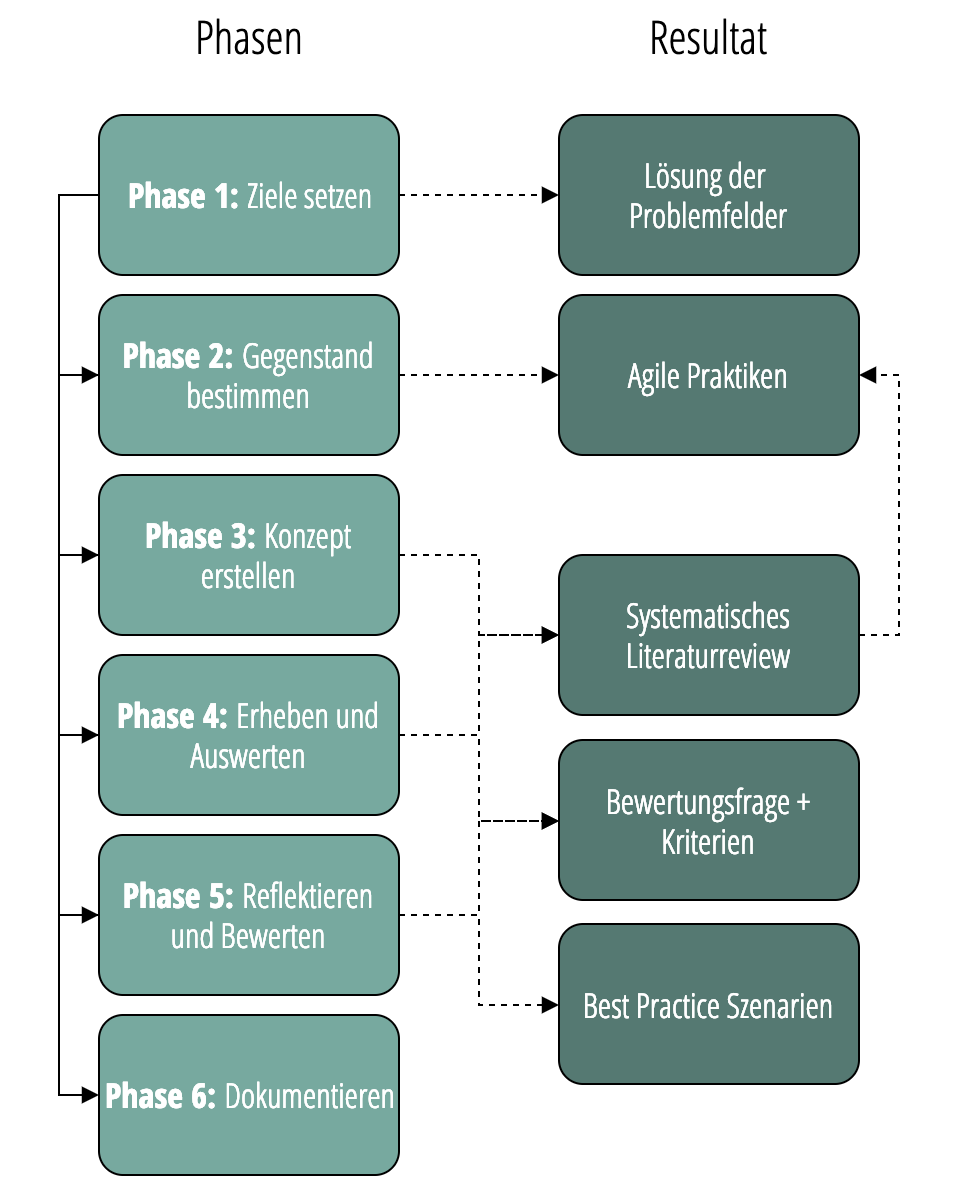
\includegraphics[width=0.6\linewidth]{pics/evaluation}}
	\caption[Darstellung Evaluationsprozess]{Darstellung Evaluationsprozess (eigene Darstellung)}
	\label{fig:evaluation}
\end{figure}

Phase 3 beinhaltet den wichtigsten Punkt der Evaluation. Hierbei wurde eine genaue \textit{Evaluationsfrage} erstellt: \textit{Welche vorher definierten Problemfelder können mithilfe welcher agilen Methode angegangen werden?}. Zum Evaluationskonzept wurden zudem Kriterien zur Beantwortung der Frage bezüglich einer jeden agilen Methode gestellt. Wichtig ist hierbei, dass die Bewertung immer auf Grundlage \textit{klarer, qualitativer Aussagen} aus der in SLR 2 gefundenen Literatur beziehen muss. Eine agile Methode gilt also genau dann als anwendbar auf ein bestimmtes Problemfeld, wenn sich dies durch eine Aussage innerhalb einer Publikation belegen lässt. Dabei soll versucht werden, keine große Reihe an Aussagen aufzulisten, sondern einzelne, aber treffende Aussagen zu einem Problemfeld zu finden. Somit wurden die Suchobjekte aus SLR 2 als Bewertungsgrundlage für die dargestellte Evaluation gewählt.  Es lässt sich erkennen, dass die Bewertung auf Grundlage rein qualitativer Daten beruht.

Phase 5 und 6 finden sich im vorliegenden Kapitel wieder. Systematisch soll für jede aufgeführte agile Methode eine kurze Darstellung platziert werden und jeweils anschließend die Bewertung auf Grundlage der Aussagen vorgenommen werden. Als Ergebnis dessen werden Best Practice Szenarien für den Einsatz der einzelnen agilen Methoden erstellt, um zusammenfassend darzustellen, in welchem Rahmen sich die Methoden einsetzen lassen.


\section{Literaturübersicht}

% - tabellarische Übersicht, Fallstudien + allgemeine Sekundäre Literatur
% - Inhaltsangabe jeder Arbeit (Zusammenfassung)

Um die Konsistenz mit dem ersten SLR  zu wahren  und außerdem eine Übersicht über die erschlossene und  gefilterte Literatur zu geben, soll diese im folgenden kurz beschrieben werden. In  \ref{tab:overviewliterature2}, \ref{tab:overviewliterature2-2} und \ref{tab:overviewliterature2-3} im Anhang findet sich die  gesamte Übersicht der für SLR 2 genutzten Literatur.

Wie bereits angeklungen wurden für das zweite systematische Literaturreview insgesamt 32 Publikationen genutzt. Jede dieser mussten zu mindestens innerhalb gesondert aufgeführter Kapitel Fallstudien über den Einsatz agiler Praktiken im Transformationsprozess beinhalten, oder explizite Handlungsempfehlung in diesem Kontext bieten. Nachfolgend soll jede Publikation kurz beschrieben werden.

\citeA{fuchs_adapting_2019} schildert in seinen Ausführungen insgesamt 4 Fallstudien zu internationalen Großunternehmen, wobei die Daten zu den untersuchten Unternehmen anonymisiert wurden. In allen Fallstudien ist ein klarer Bezug zum Einsatz von Agilität innerhalb der Organisationsentwicklung im Kontext der Digitalen Transformation sichtbar. Interessant ist in den Ausführungen besonders, dass eine klare Verbindung zwischen Einbettung agiler Methoden, beispielsweise im Produktmanagement, und gesamtorganisationellen Veränderungen zu erkennen war \todo{Zitat?}.

Ein starken Bezug zum Einsatz von \textit{Design Thinking} als ein Beispiel für eine agile Methode haben die 10 Fallstudien in der Arbeit von \citeA{prasad_adopting_2018}. Sie zeigen Best Practices  für den Einsatz dieser Methode, sowie die Wichtigkeit von Kundenorientierung in der Produktentwicklung.

Ein weiteren Bezug zur Organisationsentwicklung liefert \citeA{alawairdhi_agile_2016} in seinen Ausführungen. In den zwei geschilderten Fallstudien wird verdeutlicht, wie bestimmte agile Methoden als Change Management Instrumente angewandt werden und welchen Beitrag sie leisten können.

\citeA{mikalsen_agile_2018} beschreiben in ihrem Beitrag eine konkrete Fallstudie über die Digitale Transformation mithilfe agiler Methoden. Sie verdeutlichen, dass der Transformationsprozess stark mit dynamischen Veränderungen einhergeht, die dauerhaft zu berücksichtigen seien.

Eine Umfrage zum Stand der Digitalisierung innerhalb der öffentlichen Verwaltung in Deutschland stellten \citeA{looks_agile_2018} zusammen. Es wird eine generelle Haltung der Beschäftigten zum Einsatz agiler Methoden in Projekten abgefragt. An der Umfrage nahmen insgesamt 38 Personen teil.

\citeA{kilu_agile_2019}  stellen in ihren Ausführungen eine Fallstudie aus der Bankenbranche vor. Es werden Vorteile und Herausforderungen beim Einsatz agiler Methoden in Unternehmen dargestellt.

Eine großangelegte Studie zur Wechselwirkung zwischen Agilität, DevOps im Speziellen und der Digitalen Transformation thematisieren \citeA{drilling_agilitat_nodate} in ihrer Arbeit. Insgesamt nahmen an der Studie 1770 Verantwortliche in Unternehmen aus 21  Ländern und 10 verschiedenen Branchen teil. Einer der Kernresultate dieser Studie ist es, dass vor allem im deutschsprachigen Raum eine große Mehrheit den Einsatz agiler Methode als erfolgsentscheidendes Kriterium der Digitalen Transformation ansehen.

Weniger die Beschreibung einer Fallstudie, sondern vielmehr einen SLR von insgesamt 42 Fallstudien zum Thema der Agilen Transformation führen \citeA{dikert_challenges_2016} in ihrem Beitrag auf. Im Kern geht es vordergründig um die Herausforderungen der Skalierung agiler Methoden auf einen gesamtorganisationellen Kontext.

\citeA{paasivaara_communities_2014} schildern in ihrer Publikation eine Fallstudie zur Skalierung agiler Methode im großen Unternehmenskontext. Es wird die besondere Rolle von Scrum im Bezug auf kontinuierliche Verbesserungsprozesse dargelegt.

\citeA{chanias_digital_2018} beschreiben ebenfalls eine Fallstudie im Bereich der Digitalen Transformation unter Einsatz agiler Methoden. Im Besonderen wird aufgeführt, wie die gewählte agile Methode  beigetragen hat, bestimmte Probleme des Veränderungsprozesses zu lösen. Es werden zudem Handlungsempfehlungen ausgesprochen.

Insgesamt 15 Fallstudien aus der Handelsbranche führen \citeA{heinemann_digitale_2016} auf, darunter ebenfalls einige mit Bezug auf agile Methoden. Dabei geht es zudem um Vorteile beim Einsatz solcher Methode, gerade im Bezug auf Flexibilität und der stetigen Generierung von Marktvorteilen.

Eine großangelegte Sammlung von Fallstudien (21) über die Digitale Transformation bieten \citeA{urbach_digitalization_2018} in ihrer Arbeit. Gerade im Bezug auf den Einsatz agiler Methoden geben sie systematisch Lessons Learned, Handlungsempfehlungen und zudem weitere Problemstellen im Veränderungsprozess.

Im spezifischen Bezug auf die agile Methode des Design Thinking stellt \citeA{mihelic_embracing_nodate} einen detaillierten Erfahrungsbericht zur Verfügung. Es wird der Innovationscharakter  dieser Methode hervorgehoben und dargelegt, welchen Beitrag sie in der Generierung von Wettbewerbsvorteilen innerhalb der Digitalen Transformation bietet.

\citeA{gerster_how_2019} zeigen in Ihrem Beitrag die Adaption agiler Methoden auf einen größeren Unternehmenskontext. Dafür werden insgesamt 12 Fallstudien internationaler Großunternehmen dargestellt. Es ist vordergründig auf die Wichtigkeit von Flexibilität und Schnelligkeit innerhalb der Digitalen Transformation eingegangen und gezeigt, wie agile Methoden in diesen Bereichen unterstützen können.

Eine weitere Fallstudie für die Adaption agiler Methoden in einzelnen Bereichen von Unternehmen zeigen \citeA{anwar_agile_2016} in ihrer Arbeit. Es wird untersucht, ob agile Methode organisationelle Prozesse optimieren können.

Wie bereits in vorangegangenen Abschnitten beschrieben gibt es für eine erfolgreiche Digitale Transformation einen großen Bedarf an stetiger Innovation. Wie der Einsatz von sogenannten \textit{DevOps} als agile Methodik dieses Ziel erreichen kann zeigen die Ergebnisse von \citeA{wiedemann_implementing_2019}. Insgesamt wurden 23 Interviews mit Vertretern aus deutschen Großunternehmen geführt. Die Befragten bewegen sich rollenmäßig im technischen Bereich (beispielsweise technische Leiter, IT Manager usw.).

\citeA{paasivaara_large-scale_2018} zeigen in ihrer Fallstudie zum Thema agiler Skalierung, wie agile Methoden in einem großen Unternehmenskontext ausgedehnt werden können. Grundsätzlich sollte das Ziel erreicht werden, kontinuierliche Produkterweiterungen anzubieten. Im Rahmen dieser Fallstudie wurden insgesamt 45 halbstrukturierte Interviews  und 5 Observationen im vorgestellten Unternehmen durchgeführt.

In der Arbeit von \citeA{weinreich_lean_2016} geht es grundsätzlich nicht um die Darstellung von Fallstudien zur Thematik, sondern explizite Handlungsempfehlungen zum Einsatz agiler Methodik in der Digitalen Transformation. Es wird ein genereller Überblickt gegeben, wie die Transformation mithilfe der Agilität gelingen kann.

Insgesamt 6 Fallstudien aus der internationalen Flugbranche präsentieren \citeA{somsen_rerouting_2019} in ihrer Arbeit. Grundsätzlich wird nach Gründen gesucht, wie und weshalb bestimmte Ansätze Digitaler Transformation gescheitert sind und wie agile Methoden in anderen Fällen helfen konnten.

Im dritten Teil ihres Buches über die Auswirkungen der Digitalen Transformation in Großunternehmen schildern \citeA{oswald_shaping_2017} auch 3 Fallstudien aus diesem Bereich. In diesen wird auch auf den Einsatz agiler Methoden eingegangen. 

\citeA{shahzad_training_nodate} skizzieren in ihrem Beitrag eine explorative Studie zum Einsatz agiler Methoden im größeren Kontext. Interessant ist hierbei, dass dies innerhalb einer universitären Veranstaltung getestet wurde. Es sollte untersucht werden, wie sich die Erkenntnisse des Einsatzes agiler Methoden auf größere  Unternehmen auswirken.

Neben allgemeinen Fallstudien zum Thema der Digitalen Transformation in Deutschland zeigen die Ergebnisse von \citeA{berghaus_2016} auch den Einsatz agiler Methoden in diesem Kontext.  Es wird allgemein gezeigt, wie der derzeitige Stand der Transformation ist, welche Probleme festzustellen sind und auch welche Methoden eingesetzt wurden.

Eine weitere Übersicht zu Fallstudien innerhalb der Digitalen Transformation bieten \citeA{gassmann_digitale_2016} in ihrer Arbeit. Dabei gibt es auch Bezug zur Agilität in diesen Unternehmen. Insgesamt 11 Fallstudien aus dem deutschsprachigen Raum werden geschildert.

Keine ausgewiesene Fallstudie, aber konkrete Handlungsweisungen zum Einsatz agiler Methoden, namentlich Design Thinking, beschreiben \citeA{gurusamy_integrated_2016} in ihrer Arbeit. Es wird ein Konzept dargelegt, wie die Digitale Transformation unter Anwendung solcher Techniken angegangen werden kann.

Ebenfalls geben \citeA{klunder_becoming_2018} Handlungsempfehlungen zum Einsatz agiler Methoden in einen größerem organisationellen Umfeld. Dabei wird gesondert auf die Rolle von Softwareproduktlinien eingegangen und wie diese mithilfe der Agilität effektiv gesteuert werden können.

\citeA{laanti_agile_2017} schildert in seiner Arbeit eine Fallstudie eines Großunternehmens aus der Finanzbranche. Es geht grundsätzlich um die Agile Transformation in einem größeren Umfeld, welche Probleme auftreten können und was die Vorteile einer solchen Transformation sind.

Eine großangelegte Studie über den Einsatz agiler Methoden in einem größeren Umfeld legen \citeA{komus_status_2017} dar. Die Studie umfasst insgesamt über 1000 Teilnehmer aus 30 verschiedenen Ländern. Es wird auf Erfolge, Praktiken und Anwendungsfelder agiler Methoden in diesem Kontext eingegangen.

\citeA{hofert_agile_2018} beschreibt in ihrem Beitrag über das sogenannte agile Mindset, d.h. die Entstehung eines Kulturwandels hin zur Agilität in Unternehmen. Dabei schildert sich außerdem 4 Fallstudien aus dem deutschen Raum in diesem Kontext. 

Starken Bezug zum Thema Innovationsmanagement hat die Fallstudie von \citeA{alt_innovationsorientiertes_2017}. Sie beschreiben, wie ein Großunternehmen die agile Methodik der \textit{DevOps} einsetzt, um kontinuierliche Innovation voranzutreiben.

Eine weitere Fallstudie bieten \citeA{rodriguez_combining_2014} in ihren Ausführungen. Dabei wird auf den Einsatz agiler Methoden im Unternehmen eingegangen und wie diese von der reinen Softwareentwicklung auf einen gesamtorganisationellen Kontext geschlossen wurden.

Die Ergebnisse von insgesamt 14 Fallstudien zu Großunternehmen schildern \citeA{alahyari_exploratory_2019}. Dabei wird vor allem auf die Problematik von \textit{Verschwendung} in großen Unternehmen eingegangen und gezeigt, wie agile Methoden dieser entgegenwirken können.

Abschließend wurde die Fallstudie von \citeA{eklund_scaling_2017} für die weiteren Untersuchungen einbezogen. Es wird ein Großunternehmen aus der Mechatronik-Industrie geschildert und gezeigt, wie agile Methode in einem größeren Kontext eingesetzt werden. 

Die immer noch große Menge an (Fall-) Studien und Fachliteratur mit ausgewiesenen Handlungsempfehlungen zum Einsatz agiler Methoden innerhalb der Digitalen Transformation bieten eine breite Palette an Erkenntnissen. Nachfolgend sollen die Ergebnisse zusammengefasst und geclustert werden.

\section{Einsatz agiler Praktiken im Unternehmen}
\label{agilepractices:extractions}

% - Ergebnisse der SLR - Auflistung der genutzten Methoden

Anhand der erschlossenen Literatur sollten agile Methoden bestimmt werden, die innerhalb von Veränderungsprozessen im Kontext der Digitalen Transformation angewandt wurden. Dabei wurden alle Fallstudien sowie die Fachliteratur untersucht und wesentliche Nennungen herausgearbeitet. Oft wurden Abwandlungen einzelner agiler Methoden aufgeführt, diese wurden dann zu der klassischen Variante zusammengeführt. In  \ref{tab:clusteringslr2} und \ref{tab:clusteringslr2-2} im Anhang wird die komplette Auswertung des SLR aufgeführt. Es wird gezeigt, welche Methoden in welcher Fallstudie bzw. Fachliteratur benutzt und beschrieben werden, sowie in welchem Kontext sie angewandt wurden. 

\todo{Vielleicht  noch Tabelle mit Anwendungsgebiet - Anzahl?}

Die numerischen Ergebnissen dessen findet sich im folgenden in \ref{tab:clusteringagileshort} als Übersicht. Neben jeder einzelnen Methode wird ebenfalls die Anzahl an Nennungen innerhalb der untersuchten Literatur aufgeführt. Man erkennt hierbei sehr gut eine große Vielfalt im Einsatz von agilen Methoden. In diesem Kontext sei auf die Wichtigkeit des Kriteriums \textit{Aktualität} im Auswahlprozess des SLR verwiesen, um den gegenwärtigen Stand der Nutzung darzustellen.

\begin{table}[ht]
	\centering
	\caption{Auswertung Nutzung agiler Methoden (kurz)}
	\begin{tabular}{|c|c|}
		\hline
		\textbf{Agile Methode}& \textbf{Anzahl Nennungen} \\
		\hline
		Scrum                          & 17               \\
		Design Thinking                & 10               \\
		DevOps                         & 8                \\
		Kanban                         & 6                \\
		XP                             & 5                \\
		SAFe                           & 4                \\
		Digital Innovation Lab         & 4                \\
		Minimum Viable Product (MVP) & 2                \\
		Squads and Tribes              & 2                \\
		LeSS                           & 1                \\
		Unified Process                & 1                \\
		Communities of Practice        & 1                \\
		Holacracy                      & 1                \\
		Culture Book                   & 1                \\
		Corporate Startups             & 1                \\
		Agile Modelling                & 1                \\
		Usability Driven Development   & 1                \\
		Lean Startup                   & 1               \\
		\hline
	\end{tabular}
	\label{tab:clusteringagileshort}
\end{table}

In der Übersicht lassen sich erste Tendenzen erkennen. Oft wurde die beispielsweise Methode \textit{Scrum} genannt und benutzt, was auf eine große Schwerpunktsetzung in die Produktentwicklung schließen lässt. Die genaue Beschreibung dieser Methode wird im nachfolgenden Abschnitt vorgenommen. 

Nachfolgend kann aus Übersichtsgründen natürlich keine Beschreibung und Evaluation aller hier aufgeführten agilen Methoden erfolgen. Deswegen wurde ab der  Nennungsanzahl ``2'' eine Trennung vorgenommen. Somit werden alle Methoden mit nur einer Nennung im folgenden verworfen. Die übrig gebliebenen Methoden bieten weiterhin eine große Auswahl an möglichen agilen Methoden für den Einsatz im Transformationsprozess. Es bleibt nun als letzten, aber wichtigsten Schwerpunkt dieser Arbeit, die erarbeiteten Methoden hinsichtlich ihrer Anwendbarkeit in den Problemfeldern der Digitalen Transformation zu bewerten.

\section{Darstellung und Evaluation verschiedener agiler Methoden}

% - systematisch: erst Definition der Methode, dann Evaluation im Bezug auf die Problemfelder
% - siehe Key findings: https://docs.google.com/document/d/1QayCknP1SgspsPvXlU_FR5u0h2fNzhfQshNOrAuTiB8/edit

Nachdem im vorherigen Abschnitt eine Reihe von agilen Methoden, die innerhalb von Transformationsprozessen genutzt wurden, aufgeführt worden sind, sollen diese im folgenden systematisch kurz beschrieben und evaluiert werden. Die Reihenfolge der Bearbeitung richtet sich nach der Anzahl der Nennungen (absteigend, vgl. \ref{tab:clusteringagileshort}). Die einzelnen Beschreibungen sollen nicht zu sehr ins Detail erfolgen. Es soll ein generelles Verständnis für die jeweilige agile Methode geschaffen werden. Um die Übersichtlichkeit zu wahren, wird nach jeder einzelnen Evaluation eine kleine Zusammenfassung aufgeführt.

\subsection{Scrum}

\subsubsection{Beschreibung}

\textit{Scrum}, so wie es gegenwärtig vermehrt eingesetzt wird, ist ein Framework zur Steuerung komplexer Projekte \cite[S. 25]{wirdemann_scrum_2017}, wobei es ursprünglich innerhalb von Softwareprojekten eingesetzt wurde. ``Komplexe Projekte'', so \citeA{wirdemann_scrum_2017}, ``sind
dadurch charakterisiert, dass nicht exakt vorhersehbar ist, welchen Verlauf das Projekt nehmen wird und was in Zukunft alles passiert'' (S. 25f.). Mit Scrum wird somit versucht, ein Rahmen zu schaffen, um flexibel auf Veränderungen innerhalb eines Projektes zu reagieren. Dabei sieht man bereits einen Bezug auf die Werte der Agilität (vgl. \ref{background}).

Der Scrum-Prozess selbst besteht aus einer Vielzahl an einzelnen Komponenten. Wie bereits erwähnt wurde, ist Scrum ein Framework. Dies beinhaltet, dass ein Rahmen bereitgestellt wird, in dem Entwicklungsteams ihre eigenen und bewährten Entwicklungspraktiken einbetten können \cite[S. 27]{wirdemann_scrum_2017}. Es geht somit um das Finden einer guten Mischung zwischen den Hilfsmitteln, die Scrum selbst bereitstellt und denen, die im Unternehmen bereits verankert sind. \ref{fig:scrum} soll einen generellen Überblick über Scrum und seine Komponenten bereitstellen. Im folgenden soll nicht auf alle Komponenten, sondern nur auf einzelne, wichtige eingegangen werden.

\begin{figure}[H]
	\centering
	\fbox{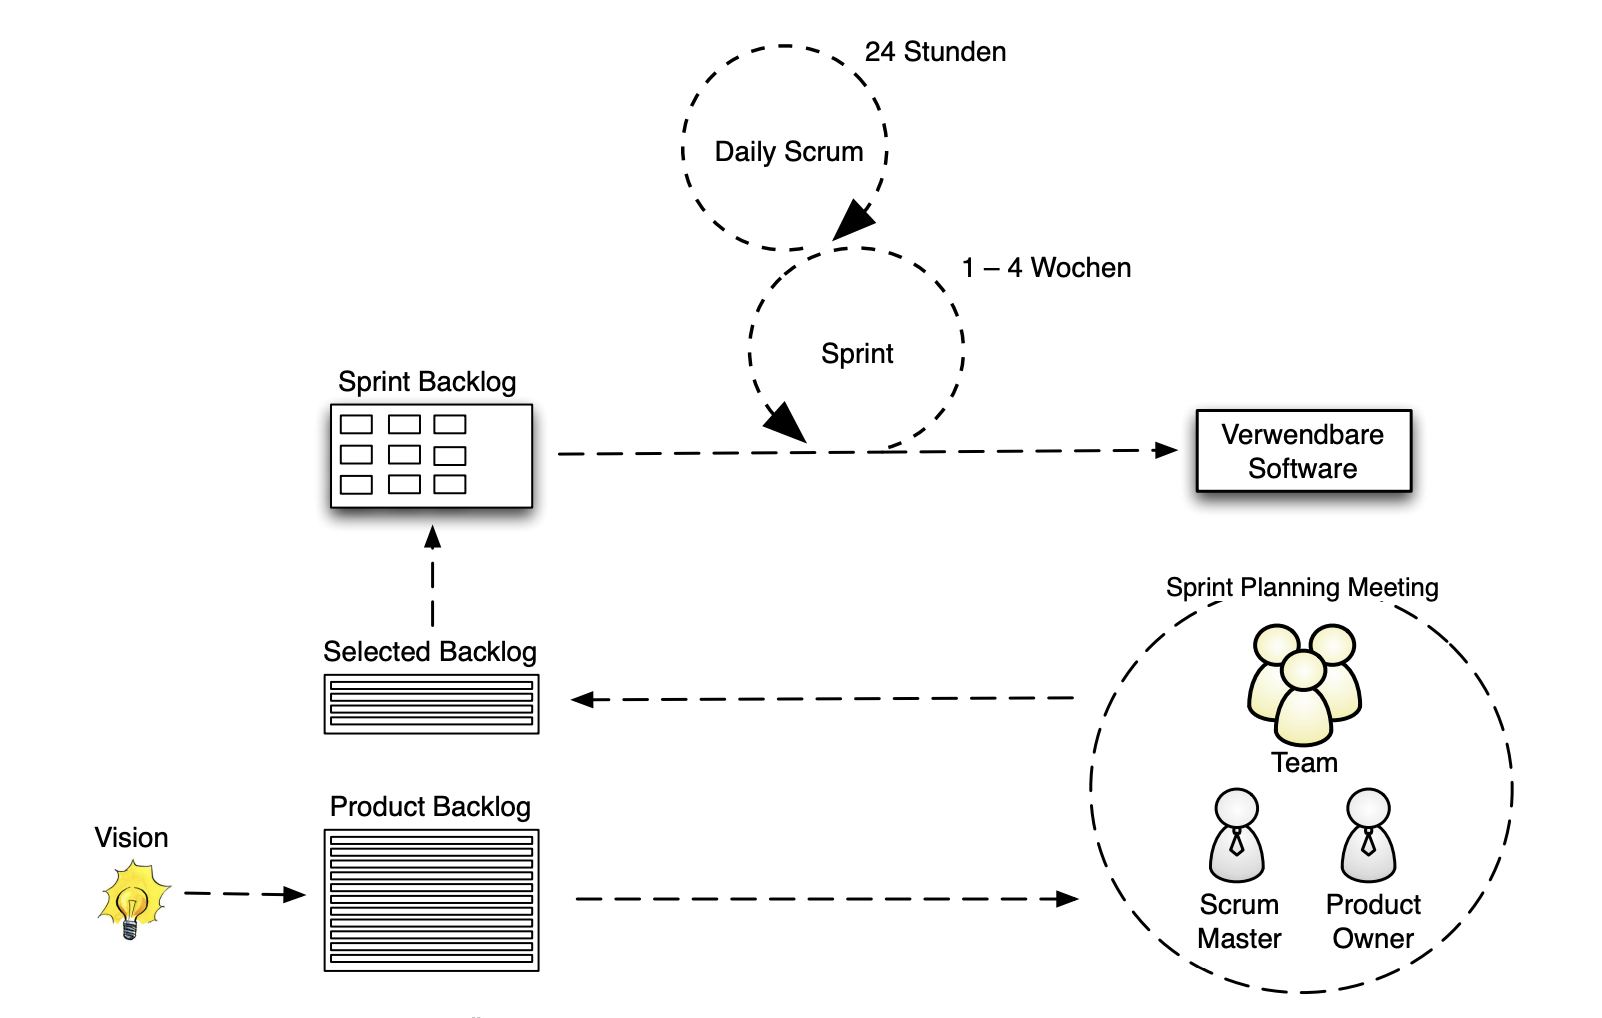
\includegraphics[width=0.9\linewidth]{pics/scrum}}
	\caption[Scrum im Überblick]{Scrum im Überblick \protect \cite[S. 29]{wirdemann_scrum_2017}}
	\label{fig:scrum}
\end{figure}

Die Übersicht lässt gut erkennen, dass man durch Scrum immer noch einen gesteuerten Prozess erhält, auch wenn versucht wird, eine gewisse  Flexibilität zu erzielen. Im Kern stehen sogenannte \textit{Sprints}. Dies sind regelmäßige Iterationen, in denen das Team selbstorganisiert arbeitet und an dessen Ende immer ein sogenanntes \textit{Increment} steht, im Falle der Softwareentwicklung eine verwendbares Produkt, was eine spürbare  Verbesserung beinhaltet \cite[S. 30]{wirdemann_scrum_2017}. Wichtig hierbei ist, dass Sprints immer eine festgelegte Länge haben. So erreicht man eine kontinuierliche Verbesserung.

Am Anfang jedes  Scrum-Prozesses steht die Definition einer \textit{Vision}. Diese `` schafft die Bedeutung [des] Handelns, indem sie klar benennt, wer das Produkt aus welchem Grund kaufen wird, welche Kundenbedürfnisse das Produkt befriedigt und worin sich das Produkt von ähnlichen, bereits existierenden Produkten unterscheidet'' \cite[S. 29]{wirdemann_scrum_2017}. Sie wird also nicht nur vom Kunden vorgegeben, sondern gemeinsam mit dem Entwicklungsteam erarbeitet. Als Ergebnis entsteht ein sogenannter \textit{Product Backlog}.

Ein Scrum-Prozess besteht aus einer Vielzahl möglicher Meetings. Diese dienen dazu, den Iterationen einen abgesteckten Rahmen zu geben. Ein Beispiel ist das \textit{Sprint Planning Meeting}. Hierbei wird der kommende Sprint vom Team vorbereitet. Es werden Aufgaben priorisiert, geschätzt und in kleinere Unteraufgaben geteilt. Am entsteht aus dem Product Backlog ein sogenannter \textit{Sprint Backlog}, der während der Iteration nicht verändert werden sollte \cite[S. 29]{wirdemann_scrum_2017}.

Das Team steht im Fokus des Prozesses. Dieses soll sich frei entfalten kommen, ist aber auch hauptverantwortlich für den Fortschritt des Projektes. Ein Scrum-Team beinhaltet mehrere Rollen, welche in \ref{fig:scrumrollen} dargestellt werden. 

\begin{figure}[H]
	\centering
	\fbox{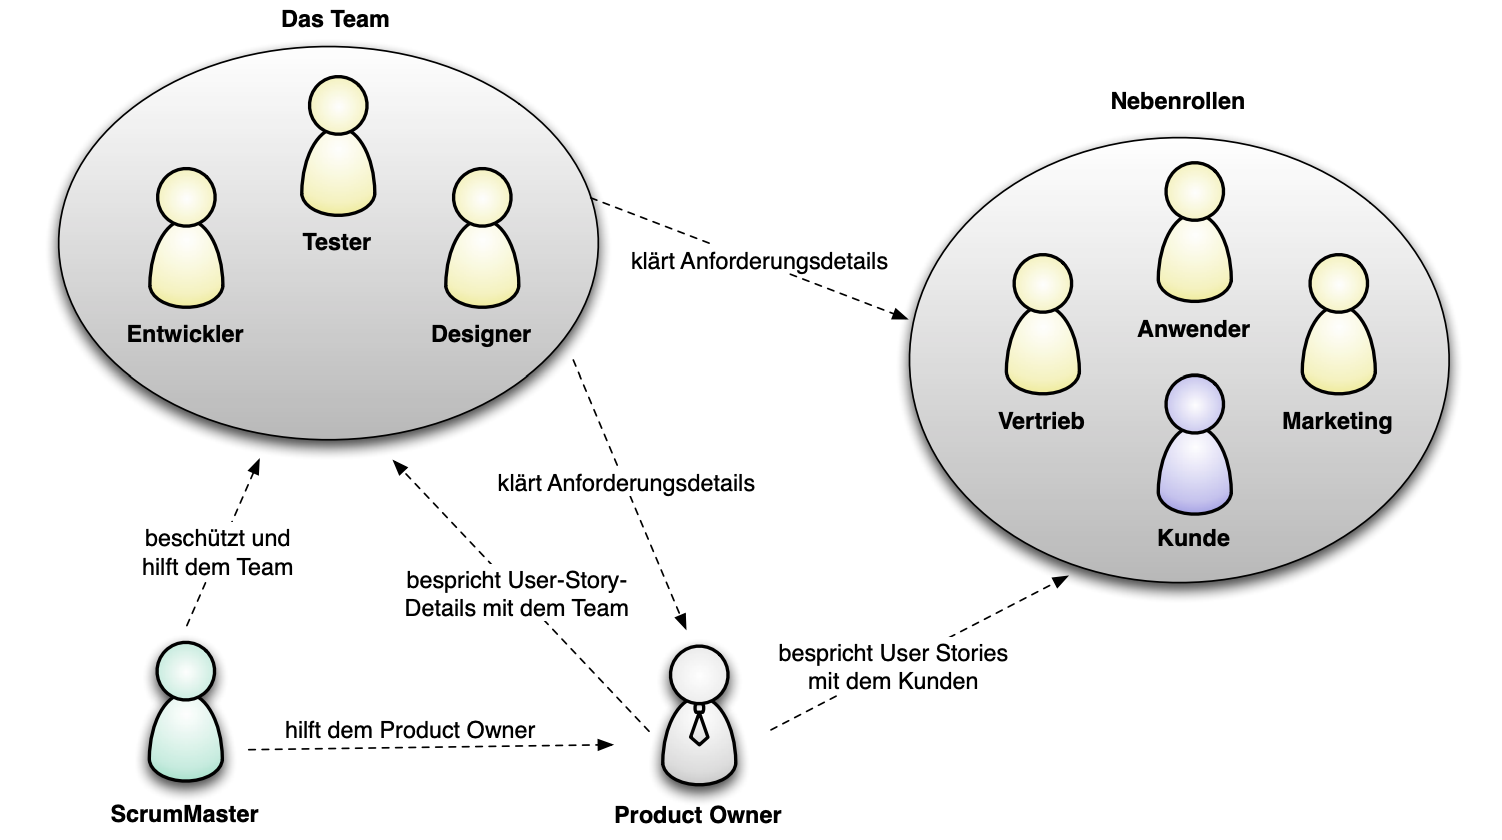
\includegraphics[width=0.9\linewidth]{pics/scrumrollen}}
	\caption[Scrum-Rollen und ihr Zusammenspiel]{Scrum-Rollen und ihr Zusammenspiel \protect \cite[S. 36]{wirdemann_scrum_2017}}
	\label{fig:scrumrollen}
\end{figure}

Im Fokus steht das eigentliche Entwicklungsteam. Dieses arbeitet im Sprint die einzelnen Aufgaben ab und sorgt am Ende für die Entstehung eines verwendbaren Produktes. Der \textit{Scrum Master} soll das Team dabei unterstützen. Er sorgt für das nötige Umfeld, um den Prozess erfolgreich zu gestalten. Der \textit{Product Owner} präsentiert die Kundenseite im Prozess. Er vermittelt mit weiteren Stakeholdern und gibt Anforderungen vor. Im klassischen Scrum-Prozess spielt der Kunde somit nur eine Nebenrolle, die aber durch den Product Owner vertreten wird. 

Ganz nach dem Wesen der Agilität folgt Scrum auch einer  Reihe von Prinzipien. Diese können von Projekt zu Projekt variieren, \citeA{wirdemann_scrum_2017} stellt eine Möglichkeit einer Gruppierung dar:

\begin{itemize}[noitemsep, topsep=0pt]
	\item Transparenz
	\item Beobachten und Anpassen
	\item Timeboxing
	\item Dinge abschließen
	\item Maximierung von Geschäftswert
	\item Teams scheitern nicht
	\item Ergebnisorientierung
\end{itemize}

Man erkennt hierbei sehr gut den Bezug auf die \textit{Agilität}. Beispielsweise spiegelt die Wichtigkeit der \textit{Transparenz} den agilen Wert der Offenheit wider (vgl. \ref{background:agile}). Man erkennt in den genannten Prinzipien aber auch das Streben nach Wirtschaftlichkeit und Erfolg (vgl. \textit{Maximierung von Geschäftswert, Timeboxing und Ergebnisorientierung}), wobei dem Team jedoch immer das nötige Vertrauen gegeben werden sollte (vgl. \textit{Team scheitern nicht}).

Scrum hat sich vermehrt in der Produktentwicklung durchgesetzt. Dies lässt auch das vorgenommene SLR 2 erkennen (vgl. \ref{tab:clusteringslr2} und \ref{tab:clusteringslr2-2} im Anhang). Spannend ist hierbei, ob und inwieweit Scrum auch in anderen Bereichen des Unternehmens eingesetzt werden kann. Scrum bietet eine große Zahl an Vorteilen. Die nachfolgende Evaluation soll zeigen, ob diese auch im Einsatz gegen die Problemfelder der Digitalen Transformation wirken.

\subsubsection{Evaluation}

Wie im Evaluationsschema (vgl. \ref{agilepractices:evaluationschema}) dargelegt, sollen nachfolgend explizite Zitate ausgewiesen werden, die belegen, welche  Problemfelder (vgl. \ref{problemfields:fields}) Scrum entgegenwirken kann. Das Ziel ist es ausdrücklich nicht, alle Problemfelder anzureißen. Es wird sich nur auf einzelne, klare Aussagen bezogen. Nachfolgend sollen diese Aussagen systematisch aufgeführt und hinsichtlich Anwendbarkeit auf bestimmte Problemfelder dargestellt werden. Englische Aussagen wurden übersetzt.

In der Untersuchung bezüglich Scrum wurde versucht, den Blick nicht nur auf reine Softwareprojekte zu setzen. Stattdessen wurde gezielt nach Aussagen gesucht, die sich auf Veränderungsprojekte beziehen, um einen stärkeren Bezug auf diese Thematik innerhalb der Evaluation zu setzen. 

\todo{Am Ende eventuell Zitate zu einzelnen Problemfeldern aus anderen Studien ergänzen}

\todo{Eventuell  andere Formattierung der Zitate?}

\citeA{fuchs_adapting_2019} führt in einer seiner Fallstudien folgende Aussage auf:

\begin{center}
	``Probleme werden offener angesprochen. Unsere Entwicklung ist viel schneller. [...] Die Transparenz ist unglaublich und hilft uns beim Engagement der Mitarbeiter.'' \cite[S. 5]{fuchs_adapting_2019}
\end{center}

Man erkennt hierbei einen ganz klaren Bezug auf das Problemfeld \textit{Fehlende Transparenz (intern und extern)}. Es zeigt sich, dass der Einsatz von Scrum dazu geführt hat, dass Mitarbeiter der Veränderung offener gegenüberstehen. Scrum lebt sehr von Offenheit, gerade auch durch das regelmäßige Zeigen von Ergebnissen. Mitarbeiter, soweit sie in den Prozess eingeschlossen werden, bekommen so ein stetiges Bild über heranwachsende Veränderungen. Interessant innerhalb der gleichen Fallstudie sind folgende Aussagen:


\begin{center}
	``Es gab Teams, die Scrum auf den ersten Blick [...] liebten, und es gab Teams, die agile Methoden vollständig ablehnten, weil ihnen eine agile Denkweise fehlten'' \cite[S. 5]{fuchs_adapting_2019}
\end{center}

\begin{center}
	 ``Motivierte Mitarbeiter wollten Teil [der agilen Initiativen] sein, um die Zukunft ihres Unternehmens zu gestalten'' \cite[S. 7]{fuchs_adapting_2019}
\end{center}


Man erkennt hier, dass Scrum keineswegs immer nur positive Auswirkungen hat. Gerade im Hinblick auf die Problemfelder des \textit{fehlenden Vertrauens, Akzeptanz und Bereitschaft} und der \textit{fehlenden frühen Einbeziehung aller Mitarbeiter} sieht man, dass auch bei der  Einarbeitung agiler Methoden, wie Scrum, Schaffung von Vertrauen notwendig ist. Die Aussagen zeigt somit aber auch, dass durch die Entstehung einer agilen Denkweise diese Probleme angegangen werden können \cite{hofert_agile_2018}. Durch eine stetige Einbeziehung in den Scrum-Prozess, der offenen Interaktion mit anderen Bereichen des Unternehmens oder durch das Anbieten von Workshops zum Erlernen der Scrum-Praktiken erreicht man einen Wachstum und Vertrauen. Man sieht hier Referenzen zum Wesen einer partizipativen Organisationsentwicklung (MOEW, vgl. Abschnitt \ref{background:change}. Im Bereich der Akzeptanz für anstehende Veränderung gab es in den untersuchten Fallstudien mehrere Referenzen zu Scrum. Beispielsweise lässt sich folgende Aussage von \citeA{dikert_challenges_2016} darstellen:

\begin{center}
	``Wenn Mitarbeiter die agilen Werte verstehen, werden sie auch verstehen, warum die Veränderung durchgeführt wird, und sich motiviert fühlen'' \cite[S. 17]{dikert_challenges_2016}
\end{center}

Es ist erkennbar, dass die Integrierung von agilen Leitgedanken, beispielsweise durch Scrum, eine generelle Akzeptanz der Veränderungen gelingen kann. Es zeigt sich, dass dadurch eine Förderung von Motivation vorgenommen werden kann. Mitarbeitern wird durch die agilen Werte im Scrum-Prozess mehr Vertrauen geschenkt, wodurch sie sich sicherer fühlen, ihren Beitrag bei den Veränderungen zu leisten.

Eine Aussage zum Problemfeld \textit{Unternehmensweite Kommunikationsprobleme} wird in der Fallstudie von \citeA{alawairdhi_agile_2016} getroffen:

\begin{center}
	``Es wurde beobachtet, dass die starke Kommunikation, klar definierte Regeln und ihre strikte Einhaltung die Projektfortschritte stark beeinflussen'' \cite[S. 4]{alawairdhi_agile_2016}
\end{center}

Diese Aussage wurde auf den Einsatz von Scrum in der Produktentwicklung getroffen. Es zeigt sich, dass die klaren Regeln und vor allem regelmäßig stattfindenden Meetings und Produktverbesserungen des Scrum-Prozesses dazu beitragen können, Kommunikationsprobleme zur verhindern oder zumindest zu bearbeiten. Es wird im Prozess klar, was in jeder Iteration vom Veränderungsprojekt oder der Produktentwicklung zu erwarten ist, wo es Probleme gab und wie daran gearbeitet werden kann. Das schafft Transparenz und verbessert die generelle interne Kommunikation. Eine weitere interessante Aussage wird in dieser Fallstudie getroffen:

\begin{center}
	``Die Zufriedenheit der Endbenutzer war die größte Errungenschaft der Aktivität'' \cite[S. 4]{alawairdhi_agile_2016}
\end{center}

Scrum arbeitet allgemein durch die Rolle des Product Owners sehr kunden- bzw. nutzerorientiert. Dies führt dazu, dass Produkte nicht am Kunden vorbei entwickelt  werden, sondern auf die eigentlichen Wünsche eingegangen wird. Man sieht hier klares Potenzial  zur Bekämpfung des  Problemfeldes der \textit{fehlenden Kundenorientierung}.

Eine weitere wichtige Aussagen treffen \citeA{anwar_agile_2016} in ihrer Fallstudie:

\begin{center}
	``Beginnend mit einem begeisterten Team, dem Durchführen richtiger Schulungen und das Aufzeigen von Erfolgsgeschichten. Dies war unser Schritt auf dem Weg zur richtigen Kultur im Unternehmen'' \cite[S. 2]{anwar_agile_2016}
\end{center}

Hier zeigt sich ein Lösungsansatz für das Problemfeld der \textit{Unternehmenskulturellen Problemen}. Durch das Begeistern der Mitarbeiter und dem Durchführen von Schulungen für Scrum wurde eine einheitliche Kultur im Unternehmen geschaffen. So wird versucht, eine funktionierende Unternehmenskultur zu etablieren, die Konflikte von vornherein beheben soll.

Im Bezug auf \textit{fehlende kontinuierliche Verbesserungsprozesse} geben \citeA{urbach_digitalization_2018} eine klare Aussage:

\begin{center}
	``Der Grundidee eines agilen Projektmanagements folgend, wurden regelmäßige Feedbackschleifen oder Überprüfungen in Abständen von etwa 2–4 Wochen geplant. [...] Einerseits wurden diese Überprüfungsmeetings genutzt, um gemeinsam das Feedback der Kunden zu reflektieren und Modifikationen und Erkenntnisse des neuesten Sprints zu demonstrieren.'' \cite[S. 146]{urbach_digitalization_2018}
\end{center}

Interessant ist diese Aussage vor allem im Hinblick, dass Scrum nicht (nur) für die reine Produktentwicklung genutzt wurde, sondern auch im Management, um die generelle Marktübersicht zu bewerten. Es lässt sich anhand der Aussage erkennen, dass die regelmäßigen Feedback-Meetings dazu beitrugen, die neuen Produkte hinsichtlich Kundenorientierung zu überprüfen, sondern auch Rückschlüsse im Bezug auf eigene Verbesserungspunkte zu gewinnen. Dadurch kommt man dem Prinzip kontinuierlicher Verbesserungsprozesse sehr nahe, allein durch das Folgen der Scrum-Regeln. Dies kann entscheidend für einen Erfolg des Transformationsprozesses sein.

\citeA{hofert_agile_2018} gibt folgende interessante Aussage: 

\begin{center}
	``Weiterhin kommt dem eine Kultur der Kollaboration entgegen, die offenbar auch auf Vorstandsebene verankert ist. Die Agilität setzte auf einem Verständnis auf, das einem kollegialen Wertecluster (bei uns cooperative style) entspricht'' \cite[S. 210]{hofert_agile_2018}
\end{center}

Wichtig hierbei zu erwähnen ist, dass in der geschilderten Fallstudie Scrum in sehr vielen Teilen des Unternehmens verankert wurde. Man setzte damit auf die Entwicklung agiler Werte bis hin zur Führungsetage. Dabei sollten vor allem Probleme gelöst werden, die dem Problemfeld der \textit{Störung durch oberes Managements} sehr nahe kommt. Im Führungskonzept soll durch eine Anwendung von Scrum ebenfalls ein Verständnis für Agilität geschaffen werden. Das soll dazu führen, dass Veränderungsprojekte aktiv durch das Management gefördert und nicht geblockt werden.

\todots

\subsubsection{Zusammenfassung}

Innerhalb der Evaluation wurden Aussagen für insgesamt \textit{8 von 21} Problemfeldern gefunden:

\begin{itemize}[noitemsep, topsep=0pt]
	\item Fehlende Transparenz (intern und extern)
	\item Fehlende frühe Einbeziehung aller Mitarbeiter
	\item Fehlendes Vertrauen, Akzeptanz und Bereitschaft
	\item Unternehmensweite Kommunikationsprobleme
	\item Fehlende Kundenorientierung
	\item Unternehmenskulturelle Probleme
	\item Fehlende Kontinuierliche Verbesserungsprozesse
	\item Störung durch oberes Management
\end{itemize}

In den meisten Aussagen spiegelt sich wieder, dass durch das Entstehen einer agilen Denkweise eine hohe Transparenz und Motivation im Unternehmen geschaffen werden kann. Die Einführung von Scrum in vielen Bereichen des Unternehmens hat in vielen Fällen dazu geführt, dass alle Mitarbeiter ein neue Unternehmenskultur vermittelt bekommen und somit aktiv in den Veränderungsprozess eingebunden wurden. Es entstand ein Gefühl der Zugehörigkeit, die Motivation für anstehende Veränderungen auf- und somit Blockaden abbaut. Nicht alle Problemfelder konnten durch Aussagen referenziert werden. Jedoch lässt sich erschließen, dass Scrum viele Ansatzpunkte liefert, um viele der in \ref{problemfields} erarbeiteten Probleme innerhalb der Digitalen Transformation anzugehen.

\subsection{Design Thinking}

\subsubsection{Beschreibung}

Die Untersuchungen in \ref{agilepractices:extractions} haben ergeben, dass \textit{Design Thinkin}g als zweit häufigste agile Methode genannt wurde. Im Gegensatz zum vorher beschriebenen Scrum richtet sich Design Thinking weniger in die eigentliche Produktentwicklung. Es geht hier um grundsätzliche Ansätze, Ideen zu generieren.

``Design Thinking leitet an, den Blick weit zu öffnen, um zu verstehen, was Menschen in bestimmten Situationen wirklich brauchen und was ihre Welt voranbringt''  schreiben \citeA{meinel_design_2016}. Der Ansatz sei geprägt von offener Zusammenarbeit multidisziplinärer Teams, um Innovationen zu entwickeln (ebenda, S. 1).  Somit ist Design Thinking als Prozess zur Generierung von neuen, innovativen Ideen zu verstehen, in allen Arten von Projekten. \citeA{lewrick_design_2018} erwähnen die Methode sogar als ein Weg, ``die Digitale Transformation von Unternehmen zu initiieren'' (S. 2). Demnach nutzen viele Unternehmen Design-Thinking-Workshops als ersten Startpunkt für den Transformationsprozess (ebenda).

Das klassische Design Thinking besteht aus vier grundsätzlichen Komponenten, die nachfolgend aufgelistet werden (nach \citeA{lewrick_design_2018}):

\begin{itemize}[noitemsep, topsep=0pt]
	\item Design-Prozess
	\item Design Thinking Mindset
	\item Arbeiten in interdisziplinären Teams
	\item kreative Räumlichkeiten
\end{itemize}

Nachfolgend auf die einzelnen Komponenten kurz eingegangen werden. Der grundsätzliche \textit{Design-Thinking-Prozess} besteht aus 6 aneinander gekoppelter Phasen. Diese werden in \ref{fig:designthinking} dargestellt. Zunächst geht es darum, ein generelles Verständnis über das Problem zu gewinnen. In ihr sollen Bedürfnisse, Ziele und Herausforderungen des anstehenden Projekts definiert werden \cite[S. 2]{lewrick_design_2018}. Anschließend werden vom Problem betroffene Personengruppen beobachtet. Das Ziel ist es, den IST-Zustand zu definieren.

\begin{figure}[H]
	\centering
	\fbox{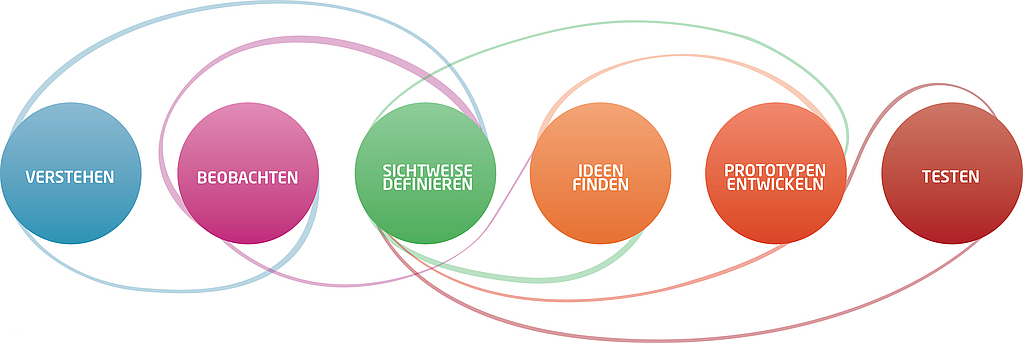
\includegraphics[width=0.9\linewidth]{pics/designthinking.jpeg}}
	\caption[Übersicht Design Thinking Prozess]{Übersicht Design Thinking Prozess \protect \footnotemark}
	\label{fig:designthinking}
\end{figure}
\footnotetext{Quelle: HPI Academy, online: \url{https://hpi-academy.de/design-thinking/was-ist-design-thinking.html}}

In einem dritten Schritt werden die Beobachtungen auf die Perspektive des einzelnen Nutzers heruntergebrochen. Es kommen ``der Ethnologie verwandte Methoden zum Einsatz, um im Kontakt mit Betroffenen ein interessantes Problem aufzuspüren``\cite[S. 3]{meinel_design_2016}. Es soll sich eine klare Fragestellung für die anstehende Ideenfindung finden. In dieser werden dann verschiedenste Kreativitätstechniken wie beispielsweise Brainstorming eingesetzt, um Lösungen für das Problem zu finden. Anhand dieser Ideen werden dann erste Prototypen erstellt, die anschließend mit dem Nutzer getestet werden. Das Ziel ist es, diese Prototypen dauerhaft mit dem Nutzer zu evaluieren und zu verbessern, bin eine optimale Lösung gefunden wurde.

Wie Scrum folgt Design Thinking auch bestimmten Werten. Es gibt eine Vielzahl dieser, so dass auf eine gesonderte Aufzählung im Folgenden verzichtet werden soll. Ein Beispiel für das \textit{Mindset} ist es, Empathie mit dem Nutzer aufzunehmen. Dadurch sollen Empfindungen und Wünsche besonders berücksichtigt werden, um die Kundenorientierung zu erhöhen \cite[S. 3]{lewrick_design_2018}. Ein weiterer Wert des Design Thinking ist die iterative Reflektion des eigenen Handelns und der erstellten Prototypen. Es soll hiermit ein kontinuierlicher Lernprozess erzielt werden \cite[S. 3]{lewrick_design_2018}. 

\begin{figure}[H]
	\centering
	\fbox{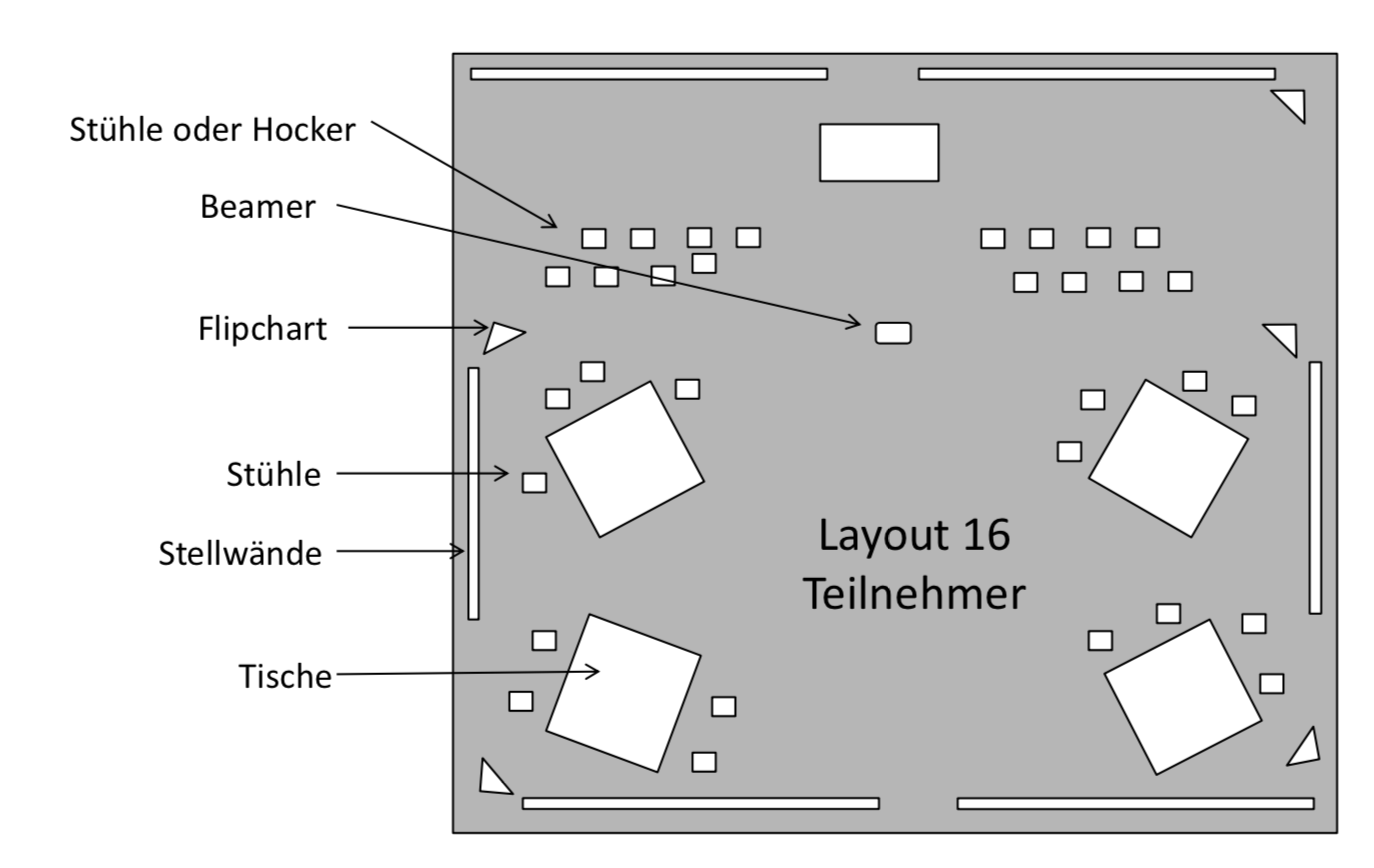
\includegraphics[width=0.9\linewidth]{pics/designthinkingroom}}
	\caption[Layout eines Design Thinking Raums]{Layout eines Design Thinking Raums \protect \cite[S. 4]{lewrick_design_2018}}
	\label{fig:designthinkingroom}
\end{figure}

Eine weitere wichtige Komponente für das Design Thinking ist das \textit{Arbeiten} in interdisziplinären Teams. In der Teamzusammenstellung wird darauf geachtet, Mitglieder aus unterschiedlichen Herkünften zu integrieren. Dies ``können beruflicher Art sein, aber auch kulturelle, nationale oder einfach nur Alters- und Geschlechtsunterschiede'' \cite[S. 3]{lewrick_design_2018}. Es geht grundsätzlich darum, einen vielseitigen Blick auf die Problematik zu bekommen.

Wichtig ist auch die Arbeit in \textit{kreativen Räumlichkeiten}. Um innovative Ideen zu entwickeln, bedarf es einer flexiblem Arbeitsfläche und Möglichkeiten zur kreativer Entfaltung. Beispielsweise können Flipcharts oder flexibles Mobiliar aufgestellt werden. \ref{fig:designthinkingroom} zeigt ein Beispiel für den Aufbau eines solchen Raums. Man erkennt hier keine starren Sitzstrukturen, sondern freier Raum für flexible Zusammenarbeit.

Nach \citeA{meinel_design_2016} sei auch die richtige Arbeitsatmosphäre entscheidend. Demnach haben sich ``das Einebnen von Hierarchieunterschieden, der Abbau von Ängsten vor dem Scheitern von Ideen, die Einführung konstruktiver Kritikformen, der Aufbau einer Kooperationskultur sowie die Unterstützung einer gelockerten Stimmungslage erwiesen'' (S. 5).

Design Thinking beschäftigt sich grundsätzlich mit einem Prozess innovativer Ideenfindung. Man sieht, dass bestimmte Werte wie Offenheit und Empathie eine wichtige Rolle spielen. Das können Ansatzpunkte zur Bekämpfung der Problemfelder in der Digitalen Transformation sein. Ob und inwieweit dies zutrifft, soll nachfolgend evaluiert werden.

\subsubsection{Evaluation}

Nachfolgend sollen wieder relevante Aussagen aus der untersuchten Literatur aufgeführt werden, die im Bezug auf die erarbeiteten Problemfelder der Digitalen Transformation stehen. \citeA{prasad_adopting_2018} geben folgende Aussage vor: 

\begin{center}
	``Am Ende des Tages hängt Sieg oder Niederlage von der Kundenerfahrung ab. [...] Customer Journeys werden verwendet, um zu verstehen, wie ein Benutzer das System verwendet, Erfahrung mit dem System macht und es werden Klarstellungen bei Grauzonen vorgenommen'' \cite[S. 3]{prasad_adopting_2018}
\end{center}

Hier gibt es einen klaren Bezug auf das Problemfeld der \textit{fehlenden Kundenorientierung}. Design Thinking bietet eine Reihe von Werkzeugen, um direkt mit dem Kunden an Produkten zu arbeiten und Ideen aus Sicht der Nutzer mit einfließen zu lassen. Die Erfüllung von Nutzerbedürfnissen steht hierbei im Fokus. Deswegen ist Design Thinking prädestiniert für die Bekämpfung dieses Problemfeldes. Den Bezug auf Kundenorientierung bot nahezu jede einzelne Fallstudie, die Design Thinking benutzte. Dies zeigt die Wichtigkeit dieser Thematik im Design-Thinking-Prozess.

\citeA{mihelic_embracing_nodate} geben folgende interessante Aussage:

\begin{center}
	``Erwartungsmanagement war die erste große Herausforderung, die wir durchlaufen mussten. Es ist schwierig, Menschen über organisatorische Änderungen zu informieren. [...] Deswegen ist Design Thinking von Vorteil. Es gibt sehr schnelle Antworten in praktisch keiner Zeit.'' \cite{mihelic_embracing_nodate}
\end{center}

Dies gibt einen Bezug auf gleich zwei der genannten Problemfeldern. Zum einen beschreibt es einen möglichen Einfluss auf die \textit{fehlende frühe Einbeziehung aller Mitarbeiter}. Design Thinking ist gerade darauf angelegt, viele Mitarbeiter aus unterschiedlichen Bereichen zusammenzubringen und gleichermaßen in ein Veränderungsprojekt miteinzubeziehen. Zum anderen wirken die Werte von Design Thinking gegen das Problem der \textit{fehlenden Transparenz (intern und extern)}. Die Aussage zeigt, dass Design Thinking einen großen Anteil am Erwartungsmanagement nach innen und außen haben kann. Es werden transparent Fortschritte präsentiert und es klar, in welchem Stand sich die fortschreitende Veränderung befindet.

Über das Problemfeld der \textit{fehlenden kontinuierlichen Verbesserungsprozesse} treffen \citeA{urbach_digitalization_2018} folgende Aussage:

\begin{center}
	``Nach einem Test-and-Learn-Ansatz werden Ideen frühzeitig getestet, um zu sehen, ob sie funktionieren. Wenn nicht, wird die Idee schnell verworfen und eine neue Idee ausprobiert'' \cite[S. 369]{urbach_digitalization_2018}
\end{center}

Regelmäßige Feedback-Schleifen gehören zum Kern des Design-Thinking-Prozesses (vgl. Prozessphasen Prototypen entwickeln und Testen). Man erreicht hierdurch, dass immer wieder neue Ideen ausprobiert werden, überarbeitet oder verworfen werden. Konzepte werden regelmäßig überprüft und Fehler fortwährend ausgeschlossen. Der eigentliche Veränderungsprojekt erhält so eine kontinuierliche Verbesserung hin zu einer optimalen Umsetzung.

\citeA{weinreich_lean_2016} führt in seiner Arbeit folgende Aussage auf:

\begin{center}
	``Design Thinking [...] bietet eine einfache Bewertungsmethode für Innovationen. Damit eine digitale Innovation erfolgreich wird, muss sie drei Qualitäten aufweisen: Erwünschtheit (Desirability), Machbarkeit (Feasibility) und Wirtschaftlichkeit (Viability). [...] Innovationen, die alle drei Qualitäten aufweisen, sind langfristig überlebensfähig'' \cite[S. 207f.]{weinreich_lean_2016}
\end{center}

Design Thinking ist für das Innovationsmanagement in Unternehmen ausgelegt. Deswegen ist es nicht verwunderlich, dass diese Methode dabei helfen kann, das Problemfeld der \textit{fehlenden Innovationskultur} anzugehen, innerhalb des Unternehmens neue Innovationen zu entwickeln und gegenwärtige Trends der Digitalisierung aufzugreifen. In diesem Zusammenhang steht auch, zumindest teilweise, das Problemfeld des \textit{fehlenden technischen Know-Hows}. Durch Design Thinking erhält man eine einfache Möglichkeit, technische Neuerungen kennenzulernen, zu evaluieren und ins Geschäftsmodell einzubinden.

Lösungsansätze für ein weiteres Problem lässt sich durch folgende Aussage von \citeA{oswald_shaping_2017} referenzieren:

\begin{center}
	``Da Business und IT von allen Seiten vertreten waren, konnte dieses Team seine funktionalen, disziplinären Fähigkeiten und sein Know-How nutzen, um die Zusammenarbeit inspirierend, wertvoll und lohnend machen'' \cite[S. 215]{oswald_shaping_2017}
\end{center}

Ein erarbeitetes Problemfeld war das der \textit{Konflikte zwischen IT und Business}. Durch den Ansatz interdisziplinärer Teams im Design Thinking können beide Seiten in Projektteams zusammengebracht werden. Es kann eine gemeinsame Sprache gefunden werden, um Missverständnisse Beiseite 
zu räumen und das Team bestehend aus beiden Seiten zu vereinen.

\todots

\subsubsection{Zusammenfassung}

In den Untersuchungen hinsichtlich Design Thinking konnten eine ganze Reihe an Problemfeldern identifiziert werden, die durch Nutzung der Methode angegangen werden können. Insgesamt wurden Aussagen für \textit{7 der 21} Problemfeldern gefunden:

\begin{itemize}[noitemsep, topsep=0pt]
	\item Fehlende Kundenorientierung
	\item Fehlende frühe Einbeziehung aller Mitarbeiter
	\item Fehlende Transparenz (intern und extern)
	\item Fehlende kontinuierliche Verbesserungsprozesse
	\item Fehlende Innovationskultur
	\item Fehlendes technisches Know-How
	\item Konflikte zwischen IT  und Business
\end{itemize}

Wieder wurden innerhalb der Untersuchung mehrere Aussagen für einzelne Problemfelder gefunden. Es wurden jeweils nur einzelne, treffende aufgeführt. Viele Aussagen zeigen, dass die klassischen Wesensmerkmale des Design Thinking vorteilhaft in der Implementierung im Unternehmen waren. Gerade der Schwerpunkt auf Kundenorientierung, den Aufbau von interdisziplinären Teams, die Förderung von Kreativität und die offene Fehlerkultur haben viele positive Einflüsse auf den Verlauf des Transformationsprozesses.
 
\subsection{DevOps}

\subsubsection{Beschreibung}

Die Methode des \textit{DevOps} wurde in insgesamt 8 untersuchten Publikationen genannt. Bei der Bezeichnung handelt es sich um eine Verkürzung und Zusammensetzung der beiden englischen Wörter \textit{Development} (Entwicklung) und \textit{Operations} (Betrieb) \cite[S. 23]{alt_innovationsorientiertes_2017}. In klassischen Organisationen arbeiten beide Abteilungen generell strikt voneinander getrennt und mit verschiedenen Zielstellungen. Dies kann innerhalb der Digitalen Transformation zu Verständigungsproblemen und Konflikten zwischen diesen beiden führen, was bereits im Problemfeld der \textit{Konflikte zwischen IT und Business} beschrieben wird.


\begin{figure}[H]
	\centering
	\fbox{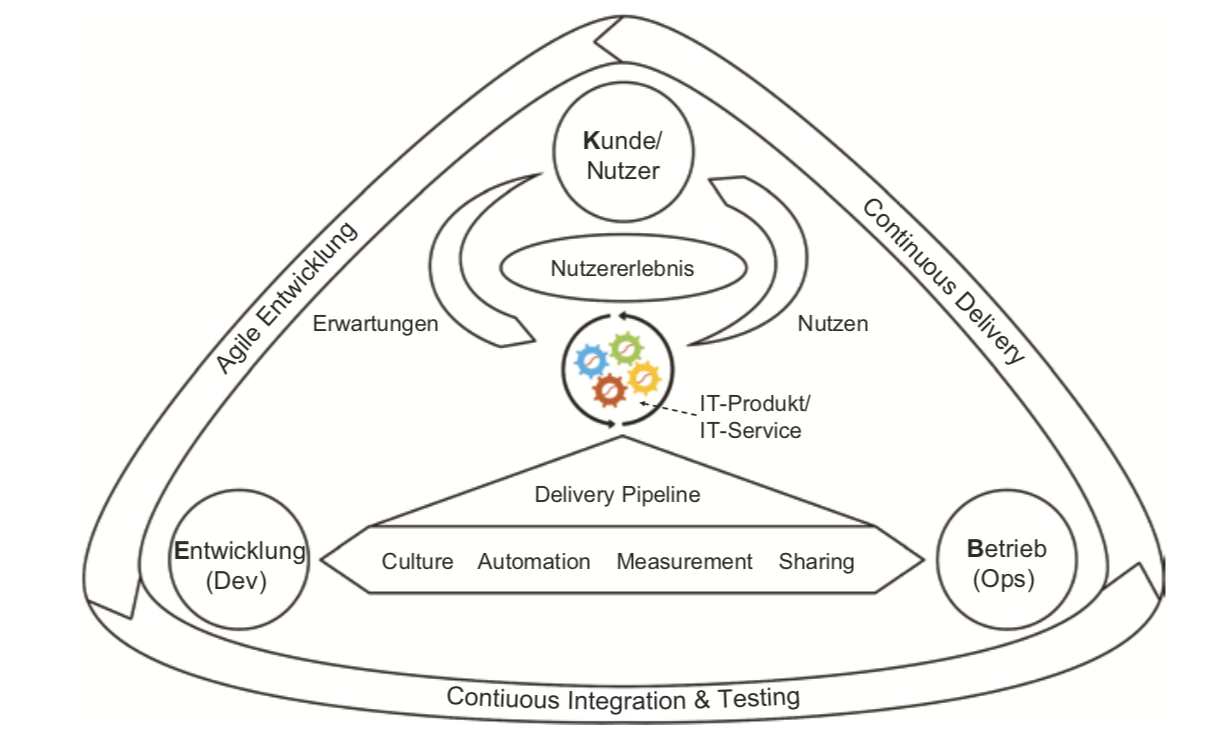
\includegraphics[width=0.7\linewidth]{pics/devops}}
	\caption[Übersicht zur Methodik DevOps]{Übersicht zur Methodik DevOps \protect \cite[S. 28]{alt_innovationsorientiertes_2017}}
	\label{fig:devops}
\end{figure}

Nach \citeA{alt_innovationsorientiertes_2017} beinhaltet die Begrifflichkeit DevOps ``eine Sammlung von Techniken, Prozessen und Tools, die darauf abzielt, typischen Problemen in der Zusammenarbeit von Entwicklungs- und Betriebseinheiten entgegen zu wirken und in der Konsequenz das Kundenerlebnis bzw. die Kundenzufriedenheit zu verbessern'' (S. 24). DevOps ist somit kein definierter Prozess, wie er teilweise bei Scrum zu finden ist, sondern bietet Hilfestellungen zur Vernetzung der beiden Geschäftsbereiche. Eine genereller Überblick über die Methodik wird in der \ref{fig:devops} dargestellt.


Die Abbildung lässt die enge Verzahnung zwischen Entwicklung und Betrieb zur Generierung einer starken Kundenorientierung erkennen. Beeinflusst wird der Einsatz von DevOps durch eine Reihe von Komponenten. Innerhalb der Produktentwicklung wird üblicherweise auf agile Prinzipien gesetzt. Daneben existieren die Prinzipien der \textit{Continuous Delivery, Integration und Testing}. Dies beinhaltet im Wesentlichen, dass die entstandenen Produkte oder Projektergebnisse dauerhaft mit dem Nutzer evaluiert, getestet und verbessert werden. Man erhält somit dauernde Feedback-Schleifen, die eine stetige Verbesserung des Prozesses erlauben. \cite{alt_innovationsorientiertes_2017}.

Wie in den vorher beschriebenen Methoden Scrum und Design Thinking folgt DevOps ebenfalls bestimmten Werten. Auch hier gilt keine allgemeine Definition. \citeA{alt_innovationsorientiertes_2017} gibt eine Möglichkeit vor, die nachfolgend aufgelistet wird:

\begin{itemize}[noitemsep, topsep=0pt]
	\item Culture: Kulturwandel hin zu einer gemeinsamen Verantwortung aller Beteiligten
	\item Automation: Die Automatisierung der Prozesskette
	\item Measurement: Erstellung von Kennzahlen zur stetigen Verbesserung
	\item Sharing: Zusammenarbeit zwischen den Beteiligten
\end{itemize}

Die Methodik von DevOps zeigt einige Parallelen zum Grundwesen der Agilität. Es lassen sich bereits erste Verweise auf mögliche Lösungsansätze für die Problemfelder der Digitalen Transformation erkennen. Nachfolgend bleibt es zu betrachten, ob sich dafür präzise Aussagen finden lassen. 

\subsubsection{Evaluation}

Nachfolgend sollen Aussagen aufgeführt werden, die  im direkten Zusammenhang mit DevOps und den erarbeiteten Problemfeldern stehen. \citeA{mikalsen_agile_2018} führt folgendes aus:

\begin{center}
	``Wenn sich etwas in der Entwicklung befindet und ein Problem auftritt, kann es passieren, dass wir informell damit umgehen, indem wir mit den Entwicklern darüber sprechen, dass es anders gelöst wird'' \cite[S. 6]{mikalsen_agile_2018}
\end{center}

Hierbei sei zu erwähnen, dass diese Aussage von einem Management-Vertreter getätigt wurde. Man erkennt sofort die Verbindung zwischen Entwicklung und Business, was das Wesen von DevOps sehr gut beschreibt. Somit ist es klar, dass das Problemfeld der \textit{Konflikte zwischen IT und Business} angesprochen wird. Die Lösung solcher Probleme ist eines der Hauptaufgaben von DevOps. Die Aussage zeigt, dass Tendenzen in diese Richtung sichtbar sind.

\citeA{drilling_agilitat_nodate} geben in ihren Ausführungen folgende Aussage vor:

\begin{center}
	``84 Prozent der deutschen Unternehmen, die agile Methoden bereits anwenden, bestätigen, dass sie die Zufriedenheit ihrer Kunden steigern konnten; deutsche Unternehmen, die auf DevOps setzen, beziffern den Anstieg [...] auf 42 Prozent'' \cite{drilling_agilitat_nodate}
\end{center}

Interessant an dieser Aussage ist, dass bestimmte Erfolge explizit anhand von Studienergebnissen belegt werden konnten. Die erfolgte Studie bezog sich direkt auf den Einsatz  von DevOps. Man erkennt einen klaren Bezug auf das Problemfeld der \textit{fehlenden Kundenorientierung}. Eines der Ziele dieser Methodik ist es, ein für den Kunden optimales Produkt zu erstellen. Deswegen können DevOps direkt in dieser Problematik eingesetzt werden.

Im Bezug auf Innovationsmanagement wurde in der Arbeit von \citeA{wiedemann_implementing_2019} folgende Aussage ermittelt:

\begin{center}
	``Darüber hinaus präsentieren wir Kernkategorien, wie die Kundenperspektiven in ein DevOps-Team integriert werden können, und zeigen auf, wie Planungsbereiche die kontinuierlichen Innovationsmechanismen beeinflussen'' \cite[S. 1]{wiedemann_implementing_2019} 
\end{center}

Es zeigt sich, dass DevOps ebenfalls einen Beitrag zur kontinuierlichen Innovation im Unternehmen beitragen kann. Dies steht im Zusammenhang mit den Problemfeldern der \textit{fehlenden kontinuierlichen Verbesserungsprozesse} und der \textit{fehlenden Innovationskultur}. Dadurch dass innerhalb der Projekte dauerhaft Feedback-Schleifen vorgenommen wurden, erreichte man zum einen eine kontinuierliche Verbesserung und zum anderen das Aufkommen neuer innovativer Ideen aus dem direkten Austausch der einzelnen Abteilungen und dem Kunden.

\citeA{alt_innovationsorientiertes_2017} stellen folgende Aussage zur Verfügung:

\begin{center}
	``Die erfolgreiche Einführung von den DevOps benötigt neben einer toolgetriebenen Automatisierung einen umfassenden Wandel der Zusammenarbeitskultur'' \cite[S. 53]{alt_innovationsorientiertes_2017}
\end{center}

Die Methode DevOps kann als Ausgangspunkt für einen Kulturwandel im Unternehmen gewonnen werden. Die Werte, die diese Methodik vorgibt, können dafür sorgen, dass eine einheitliche, agile Kultur implementiert wird. Dadurch bieten DevOps Lösungsansätze für das Problemfeld der \textit{unternehmenskulturellen Probleme}.

\subsubsection{Zusammenfassung}

Insgesamt hat die Untersuchung ergeben, dass DevOps \textit{5 der 21} Problemfelder tangieren kann:

\begin{itemize}[noitemsep, topsep=0pt]
	\item Konflikte zwischen IT und Business
	\item Fehlende Kundenorientierung
	\item Fehlende kontinuierliche Verbesserungsprozesse
	\item Fehlende Innovationskultur
	\item Unternehmenskulturelle Probleme
\end{itemize}

Das Hauptziel von DevOps ist die Verbindung zwischen Business- und Entwicklungsabteilungen. Durch die Vorgabe bestimmter agiler Werte kann so ein Kulturwandel im Unternehmen angestrebt werden. Durch die dauernde Evaluation der Projektverläufe mit dem Kunden kann eine kontinuierliche Innovation im Unternehmen gelingen.

\subsection{Kanban}

\subsubsection{Beschreibung}

Ursprünglich kommt die Methodik \textit{Kanban} aus der Produktion.  Es diente als Zeitplanungssystem, das bei der Entscheidung über die Menge der zu produzierenden Waren helfen sollte. Dabei wird stets darauf geachtet, dass die Menge der gegenwärtig arbeitenden Prozesse (\textit{Work in Progress, WIP}) durch bestimmte Regularien begrenzt wird. \cite[S. 12f.]{leopold_kanban_2018}.

Dieses Prinzip wurde unter dem Schwerpunkt agiler Methodik zunehmend auf Software-, aber auch Veränderungsprojekte übernommen. \citeA{anderson_essenz_2018} führen in Bezug auf Kanban auf, dass ``es als Methode charakterisiert werden kann, die sich dadurch auszeichnet, dass man mit dem beginnt, was man gerade tut'' (S. 1). Es sei ein Katalysator für schnelle und gezielte
Veränderungen in Organisationen, die den Widerstand gegen vorteilhafte Veränderungen im Sinne der Ziele der Organisation verringern könne (ebenda). Wie bereits innerhalb anderer agiler Methoden thematisiert, werden die Vorteile von Kanban durch das Umsetzen seiner Werte erzielt. \citeA{anderson_essenz_2018} geben folgende vor:

\begin{itemize}[noitemsep, topsep=0pt]
	\item Transparenz
	\item Balance
	\item Kollaboration
	\item Kundenfokus
	\item Arbeitsfluss
	\item Führung
	\item Verständnis
	\item Respekt
	\item Vereinbarung
\end{itemize}

Man erkennt hier durchaus Parallelen zu anderen agilen Methoden, wie beispielsweise Scrum. Basierend auf diesen Werten bilden sich gängige Kanban-Praktiken, die vermehrt in Projekten angewandt werden. Beispiele für diese finden sich nachfolgend:

\begin{itemize}[noitemsep, topsep=0pt]
	\item Visualisiere
	\item Limitiere die parallele Arbeit (WIP)
	\item Manage den Arbeitsfluss
	\item Mache Prozessregeln explizit
	\item Implementiere Rückkopplungsschleifen
	\item Verbessere gemeinsam, entwickle experimentell weiter
\end{itemize}

Interessant ist hier besonders die erste Praktik der Visualisierung. Ein oft genutztes Werkzeug ist hierbei das sogenannte \textit{Kanban-Board}. Dieses wird gerade im Projektmanagement genutzt, um Aufgaben zu ordnen, zu clustern und zu priorisieren. Die Aufteilung kann hierbei stark variieren, gleich ist aber das Prinzip, dass der Fortschritt einer jeden Aufgabe von links nach rechts erkennbar ist. \cite[S. 21]{anderson_essenz_2018} Ein Beispiel eines Kanban-Boards findet sich in \ref{fig:kanban}.

\begin{figure}[H]
	\centering
	\fbox{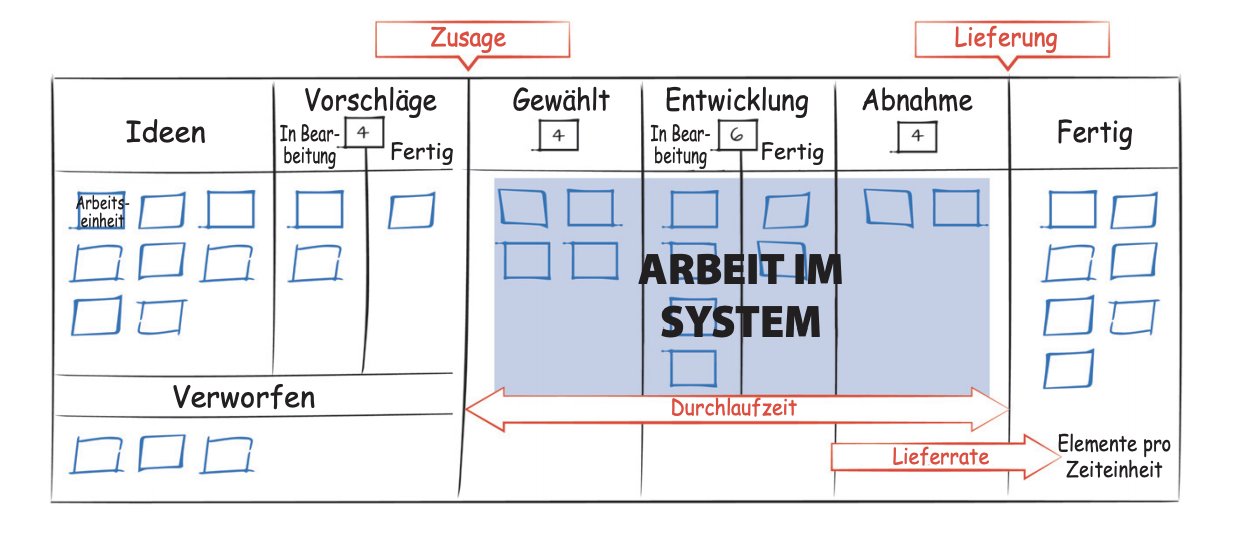
\includegraphics[width=0.9\linewidth]{pics/kanban}}
	\caption[Beispielhaftes Kanban-Board]{Beispielhaftes Kanban-Board \protect \cite[S. 15]{anderson_essenz_2018}}
	\label{fig:kanban}
\end{figure}

Kanban bietet viele Ansatzpunkte, die auch für das Change Management im Unternehmen wichtig sein kann. Inwieweit es auch dazu beitragen kann, explizite Problemfelder der Digitalen Transformation zu bearbeiten, soll nachfolgend dargestellt werden.

\subsubsection{Evaluation}

\todots

\subsubsection{Zusammenfassung}

\todots

\subsection{XP}

\subsubsection{Beschreibung}

\todots

\subsubsection{Evaluation}

\todots

\subsubsection{Zusammenfassung}

\todots

\subsection{SAFe}

\subsubsection{Beschreibung}

\todots

\subsubsection{Evaluation}

\todots

\subsubsection{Zusammenfassung}

\todots

\subsection{Digital Innovation Lab}

\subsubsection{Beschreibung}

\todots

\subsubsection{Evaluation}

\todots

\subsubsection{Zusammenfassung}

\todots

\subsection{Minimum Viable Product}

\subsubsection{Beschreibung}

Verhältnismäßig wurde die Methode des \textit{Minimum Viable Product} (MVP) in der untersuchten Literatur genannt. Diese ist ursprünglich Teil der sogenannten \textit{Lean Startup} Methode, wird aber vermehrt unabhängig davon genutzt.

Grundsätzlich wird das MVP als das minimal funktionstüchtige Produkt verstanden, was Unternehmen innerhalb ihrer Produktentwicklung in einem sehr frühen Stadium bereits auf dem Markt bringen, um schnelle Wettbewerbsvorteile zu generieren. Dadurch können Innovationen schneller umgesetzt und auf wechselnde Kundenorientierung flexibler reagiert werden. \cite{depiereux_minimum_2019}

Das Minimum Viable Product steht im Kern des im Lean Startup durchgeführten \textit{Build-Measure-Learn Feedback Loop}. Dieser Prozess wird in \ref{fig:mvploop} dargestellt. Im Grunde geht es darum, Ideen mit dem Nutzer zu generieren, daraus ein schnelles MVP zu implementieren und dieses dann direkt mit dem Nutzer zu validieren. Dadurch erhält man einen schnelleren Marktzugang und kann eine stetige Produktverbesserung herbeiführen. \cite[S. 102]{grote_fuhrungsinstrumente_2018}

\begin{figure}[H]
	\centering
	\fbox{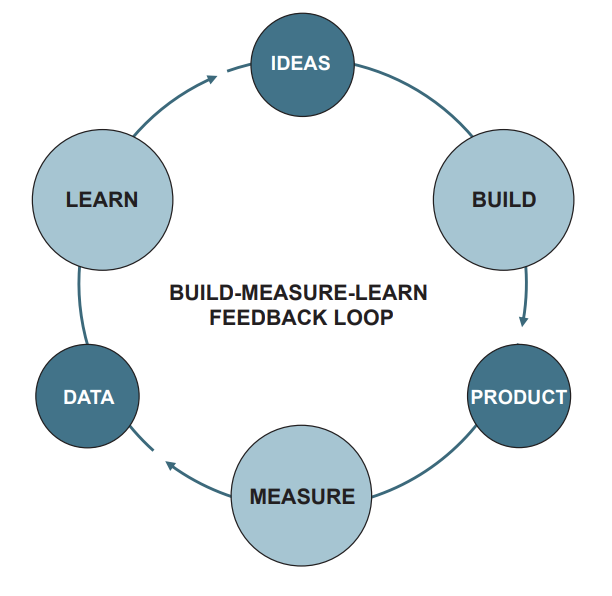
\includegraphics[width=0.6\linewidth]{pics/mvploop}}
	\caption[Build-Measure-Learn Feedback Loop als Grundlage des Minimum Viable Product]{Build-Measure-Learn Feedback Loop als Grundlage des Minimum Viable Product \protect \cite[S. 103]{grote_fuhrungsinstrumente_2018}}
	\label{fig:mvploop}
\end{figure}

Die Methode des MVP wird oft im Zusammenhang mit anderen agilen Methoden genutzt. Die Charakteristiken erinnern an das Erstellen von Prototypen im Design Thinking. Inwieweit diese Technik bei der Begegnung der Problemfelder helfen kann, soll im folgenden evaluiert werden.

\subsubsection{Evaluation}

Zwar wurde die Methodik des MVP nur in 2 der untersuchten Publikationen genannt, trotzdem lassen sich aus diesen interessante Aussagen extrahieren. Eine bieten beispielsweise \citeA{chanias_digital_2018}:

\begin{center}
	``Ein agiler Ansatz, der auf 'Versuch und Irrtum' aufbaut, ist besser als ein analytischer Planungsprozess'' \cite[S. 15]{chanias_digital_2018}
\end{center}

Hier lassen sich bereits zwei Problemfelder identifizieren. Einerseits kann das Umdenken in eine sogenannte \textit{Trial and Error} Mentalität dazu führen, dass \textit{Festhalten an verfestigten Strukturen} aufgebrochen werden kann. Man erhält ein generell neue Philosophie darüber, dass langfristige Planungen nicht immer zielführend sind, man flexibler und dynamischer in seinen Prozessen sein muss. Anderseits erhält man durch diesen Ansatz Lösungen für das Problemfeld der \textit{fehlenden kontinuierlichen Verbesserungsprozesse}. Durch den Einsatz von MVPs erhält man in regelmäßigen Abständen die Chance, Produkte direkt mit dem Nutzer zu evaluieren. Dies fördert das Einrichten von Feedback-Schleifen und somit das Entstehen einer kontinuierlichen Verbesserung. Die gleiche Fallstudie bietet eine weitere Aussage:

\begin{center}
	``Man arbeitet stark  nutzer-, aber auch innovationsorientiert'' \cite[S. 13]{chanias_digital_2018}
\end{center}

Auch hier lassen sich Lösungsansätze für gleich zwei Problemfelder finden. Zunächst bietet das MVP eine starke \textit{Kundenorientierung}, da neue Produkte schnell und dauerhaft mit dem Nutzer getestet werden. Man kann so sehr gut auf wechselnde Kundenanforderungen eingehen. Des weiteren erhält man durch das stetige Ausprobieren neuer Produktideen Ansätze zur Lösung des Problemfelds der \textit{fehlenden Innovationskultur}. Ideen werden fortlaufen mit dem Nutzer evaluiert, was neue Einflüsse in die Produktentwicklung bringt.

Eine weitere interessante Aussage führen \citeA{gassmann_digitale_2016} auf:

\begin{center}
	``Eine schnelle Time-to-Market erreicht man in der Regel durch die Entwicklung eines Minimum Viable Products (MVP)'' \cite[S. 213]{gassmann_digitale_2016}
\end{center}

Man erhält hier einen sehr starken Ansatzpunkt für das Problemfeld des \textit{Zeit - und Marktdrucks}. MVP bietet einen sehr schnellen Marktzugang. Man kann in kürzerer Zeit neue Produkte bieten, diese dauerhaft evaluieren und somit Marktvorteile generieren.

\subsubsection{Zusammenfassung}

Trotz weniger Nennungen konnten Aussagen für insgesamt \textit{5 der 21 Problemfelder} gefunden werden:

 \begin{itemize}[noitemsep, topsep=0pt]
	\item Festhalten an verfestigen Strukturen
	\item Fehlende kontinuierlichen Verbesserungsprozesse
	\item Fehlende Kundenorientierung
	\item Fehlende Innovationskultur
	\item Zeit- und Marktdruck
\end{itemize}

Die eher kleine Methode des Minimum Viable Product bietet weite Anwendungsmöglichkeiten, in jeder Facette der Produktentwicklung. Durch die schnellen Evaluationszyklen erhält man Einblicke in Kundenwünsche und kann durch den schnellen Eintritt in den Markt Vorteile gegenüber der Konkurrenz gewinnen.

\subsection{Squads and Tribes}

\subsubsection{Beschreibung}

\textit{Squads and Tribes} ist ein Ansatz zur Entstehung einer Agilen Organisation, der als erstes in der Firma \textit{Spotify} eingesetzt wurde. Er baut sich im Grunde aus Prinzipien vieler agiler Methoden auf und versucht, eine gesamte Organisation aus einzelnen Teilbereichen entstehen zu lassen. Der grundsätzliche Aufbau einer solchen Struktur wird in \ref{fig:squadstribes} dargestellt. Nachfolgend sollen die einzelnen Komponenten dieser Methodik erläutert werden. 

\begin{figure}[H]
	\centering
	\fbox{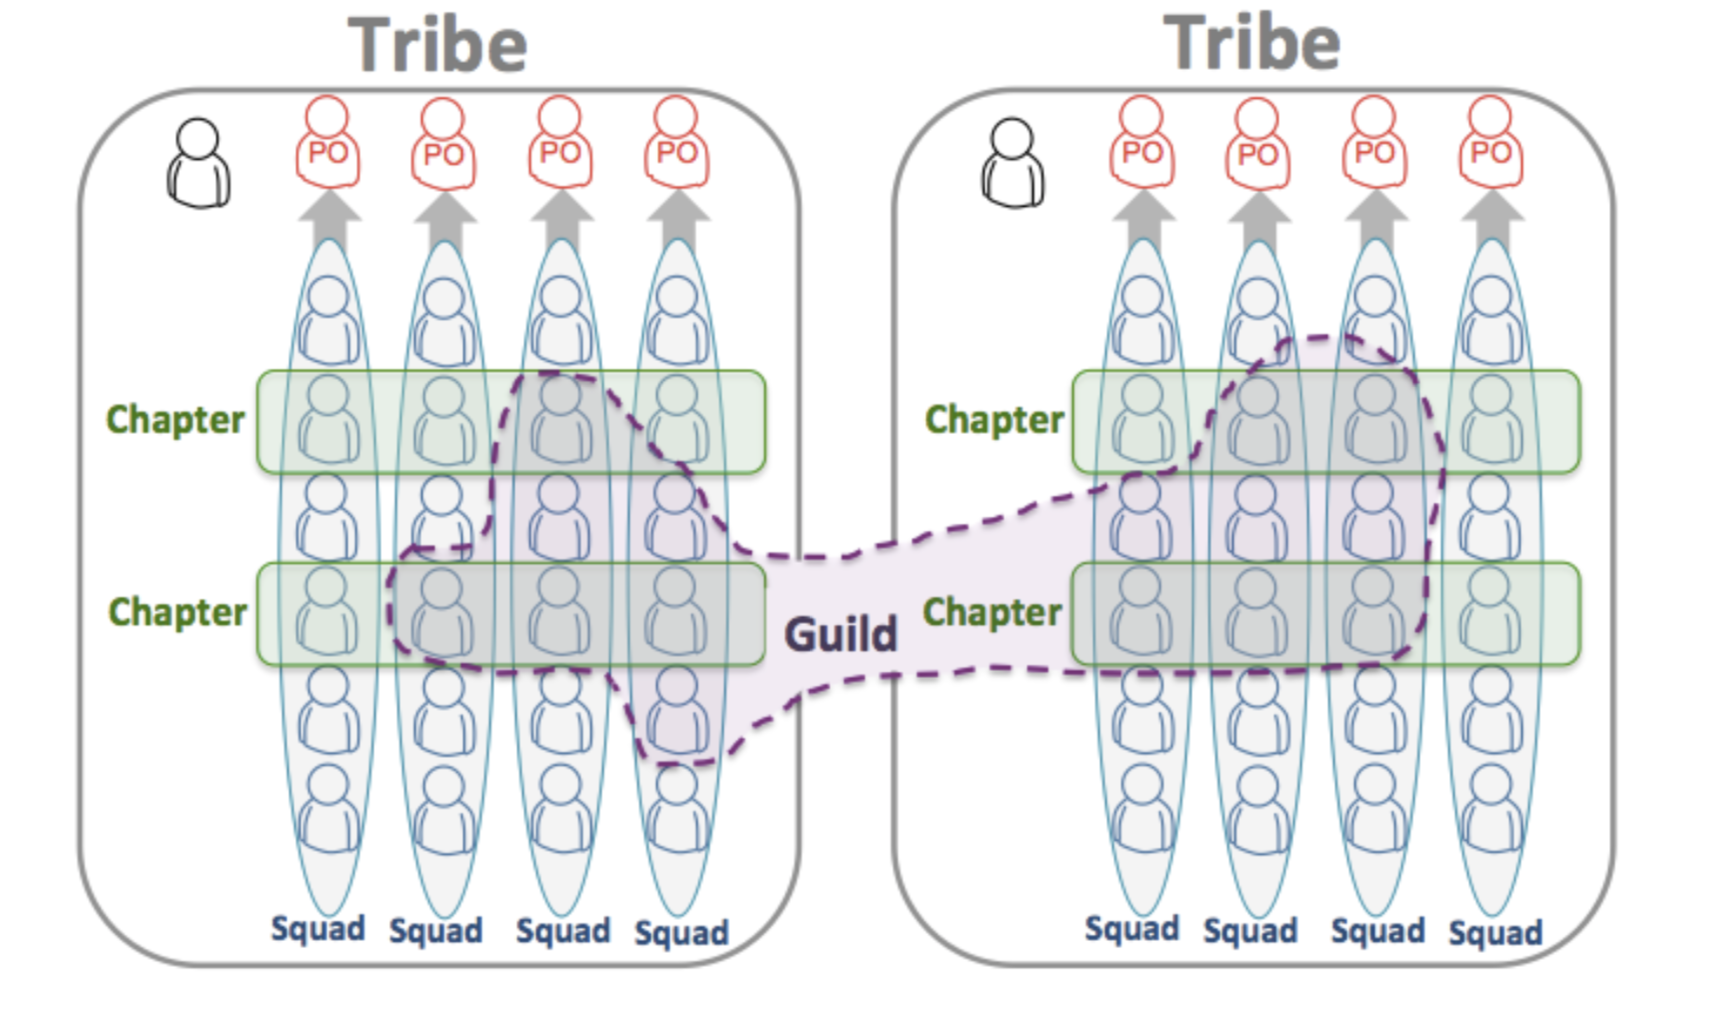
\includegraphics[width=0.9\linewidth]{pics/squadstribes}}
	\caption[Übersicht einer Squads and Tribes Organisation]{Übersicht einer Squads and Tribes Organisation \protect \cite[S. 1]{kniberg_scaling_2012}}
	\label{fig:squadstribes}
\end{figure}

Eine solche Organisation besteht im Kern aus einer Vielzahl sogenannter \textit{Squads}. Ein Squad-Team ist vergleichbar mit einem Scrum-Team, die eigenständig an einer Komponente im Projekt, ursprünglich in einem Softwareprojekt, arbeiten. Jeder Squad organisiert sich selbst und entscheidet selbst über die Wahl seiner Methoden. Manche Team nutzen Scrum, manche Kanban-Boards, manche ganz andere agile Ansätze. Squad-Teams kann man somit als Verknüpfung vieler einzelner agiler Methodiken verstehen. \cite[S. 2]{kniberg_scaling_2012}

Sogenannte \textit{Tribes} lassen sich als Verbund einzelner Squads verstehen, die in einer bestimmten zusammenhängenden Thematik arbeiten. Sie arbeiten eng zusammen, ohne eine zu strenge Hierarchie zwischen den Teams aufkommen zu lassen. In der Arbeitsorganisation im Unternehmen prägen sich Tribes meistens so aus, dass die zugehörigen Squads beispielsweise im gleichen Büro sitzen.  \cite[S. 3]{kniberg_scaling_2012}

Neben den übergeordneten Tribes gibt es andere Varianten zu Verbindungen zwischen einzelnen Squads. Einzelne Personen aus verschiedenen Squads können separate Gruppen bilden, um beispielsweise an eigenen Mini-Projekten zu arbeiten. Dies fördert das Zusammenkommen unterschiedlicher Disziplinen. Bilden sich Gruppen ausschließlich aus dem gleichen Tribe, spricht man hier von einem \textit{Chapter}, sind die Verbindungen übergreifend, erhält man ein \textit{Guild}. \cite[S. 9f.]{kniberg_scaling_2012}

Squads und Tribes bietet also eine Vielzahl von Möglichkeiten, Teams zu gruppieren. Dabei wird den einzelnen Teams völlige Freiheiten über ihre Arbeitsorganisation gegeben. Zudem erhält jeder einzelne Mitarbeiter die Möglichkeit, bereichsübergreifend tätig zu werden. Dies verhindert starre Strukturen und fördert die Kommunikation im Unternehmen. 

Um trotzdem eine Art Überwachung über die Prozesse zu gewährleisten, werden für jede der Gruppierungen Leiter eingesetzt, im Falle eines Squads beispielsweise die aus Scrum bekannten \textit{Product Owner}. Sie sind nicht als klassische Vorgesetzte zu verstehen, sondern sollen bei Problemen der Teams unterstützend wirken. Für die Förderung agiler Werte können sogenannte \textit{Agile  Coaches} eingeführt werden. Sie sorgen dafür, dass die Teams sich kontinuierlich verbessern. \cite[S. 4]{kniberg_scaling_2012}

\subsubsection{Evaluation}

Die Methodik Squads and Tribes wurde verhältnismäßig wenig  genannt, bietet aber trotzdem Ansatzpunkte für Lösungen der Problemfelder. Beispielsweise führen \citeA{heinemann_digitale_2016} folgende Aussage auf:

\begin{center}
	``Durch die hohe Autonomie in den Squads und Tribes verzichtet [das Unternehmen] auf „Economies of Scale and Scope“ zugunsten von schnellen Entscheidungen und Selbststeuerung.'' \cite[S. 98]{heinemann_digitale_2016}
\end{center}

Squads and Tribes bietet die Möglichkeit flacher Hierarchien, weswegen können Entscheidungen schneller getroffen werden können. Das bietet einen klaren Lösungsansatz für die Problematik der \textit{langsamen Entscheidungsprozesse}. Dadurch das die einzelnen Squads sich selbst  organisieren, werden bestimmte Vorgänge schneller als in einer klassischen Hierarchie durchlaufen. In der gleichen Fallstudie wird eine weitere interessante  Aussage getroffen:

\begin{center}
	``Regelmäßige Feedbackschleifen zwischen allen Squad-Mitgliedern ersetzten die Hierarchie und verbessern das Arbeitsergebnis'' \cite[S. 98]{heinemann_digitale_2016}
\end{center}

Hier erkennt man einen Bezug auf das Problemfeld der \textit{fehlenden kontinuierlichen Verbesserungsprozesse}. Die Methode bietet regelmäßige Feedback-Schleifen an, was es ermöglicht, die eigene Arbeit dauerhaft auch zwischen einzelnen Squads zu evaluieren und zu verbessern. Dies fördert eine andauernde Verbesserung des gesamten Projekts.

\citeA{gerster_how_2019} führen in ihrer Arbeit folgende interessante Aussage bezüglich den Einsatz von Squads und Tribes auf:

\begin{center}
	``Wir fanden heraus, dass innovative Geschäftsbereiche offener sind, direkt agile Strukturen zu übernehmen und eine anfängliche bimodale Einstellung zu überspringen'' \cite[S. 9]{gerster_how_2019}
\end{center}

Es zeigt sich, dass der Einsatz von Squads and Tribes die Bereitschaft der Mitarbeiter steigert. Jede einzelne Person erhält mehr Verantwortung und Vertrauen im Projekt. Dies steigert die Bereitschaft jedes Einzelnen. Somit erhält man einen Ansatzpunkt für das Problemfeld von \textit{fehlendem Vertrauen, Akzeptanz und Bereitschaft}.

\subsubsection{Zusammenfassung}

Durch die Tatsache, dass die Methode der Squads and Tribes nur vermindert erwähnt wurde, konnten nicht viele Aussagen im Bezug auf die Problemfelder gefunden werden. Trotzdem ließen sich Lösungsmöglichkeiten für \textit{3 der 21} Problemfelder identifizieren:

 \begin{itemize}[noitemsep, topsep=0pt]
 	\item Langsame Entscheidungsprozesse
 	\item Fehlende kontinuierlichen Verbesserungsprozesse
 	\item Fehlendes Vertrauen, Akzeptanz und Bereitschaft
 \end{itemize}

Es zeigt sich, dass auch diese Methodik Möglichkeiten für die Digitale Transformation bietet. Gerade durch die schnelle Dynamik der Squads lassen sich Veränderungsprozesse beschleunigen und Entscheidung schneller treffen. Jede Person des Projekts erhält gezieltes Vertrauen, was die allgemeine Bereitschaft erhöht.

\section{Formulierung agiler Best Practice Szenarien}

% - Erstellung von Thesen für Best-Practice Szenarien (im Bezug auf allen Ergebnissen von vorher, vor allen auch 4.3)
% https://docs.google.com/spreadsheets/d/1j6PUqyl1q63nIuAYo6TgqNOZqjwUseDmCFHqfY1Xj_U/edit#gid=0

\todo{Kreuzmatrix Problemfelder - agile Methode?}

Der folgende Abschnitt soll zusammenfassend die Ergebnisse des gegenwärtigen Kapitels darstellen. Durch die Evaluation der erarbeiteten agilen Methoden lassen sich Gemeinsamkeiten in deren Einsatz in Großunternehmen feststellen. Dafür soll versucht werden, anhand der Evaluationsergebnisse Leitlinien für einen erfolgreichen Einsatz agiler Methoden im Transformationsprozess zu formulieren.

\todots


